%%%%%%%%%%%%%%%%%%%%%%%%%%%%%%%%%%%%%%%%% 
% Loli Pinel del Valle
% Junio 2015
%%%%%%%%%%%%%%%%%%%%%%%%%%%%%%%%%%%%%%%%%

%----------------------------------------------------------------------------------------
%	MAIN
%----------------------------------------------------------------------------------------

\documentclass[11pt,a4paper,twoside]{book}
\usepackage[pdftex]{hyperref}
\usepackage{graphicx}
\usepackage[small]{caption}
%\usepackage[font=small,format=plain,labelfont=bf,up,textfont=it,up]{caption}
\usepackage{subfigure}
\usepackage[english]{babel}
\usepackage[utf8]{inputenc}
\usepackage{fancyhdr}
\usepackage{invuc3mlib}
\usepackage{url}
\usepackage{apacite}
\usepackage[nottoc,notlof,notlot]{tocbibind}%was commented out.
\usepackage{palatino} %math font
%\usepackage[Lenny]{fncychap}
\usepackage{colortbl}
\usepackage{indentfirst}
\usepackage{hhline}
\usepackage{mathtools}
\usepackage{amsmath}
\usepackage{pdfpages} % for incluiding pdf images
\hypersetup{  
    pdftitle={Master Thesis - Author},
    pdfsubject={Master Thesis - Author},
    pdfauthor={Author},
    pdfkeywords={keyword1} {keyword2},
    colorlinks,
    citecolor=black,
    filecolor=black,
    linkcolor=black,
    urlcolor=black, } 

\usepackage[twoside]{geometry}
\geometry{twoside, bindingoffset=1cm, papersize={210mm,297mm}, total ={135mm, 220mm}, includefoot, includehead}

\setlength{\topmargin}{0cm} 
\setlength{\headsep}{8mm}
\setlength{\marginparwidth}{20mm} \setlength{\evensidemargin}{4mm} \setlength{\oddsidemargin}{20mm}
\newcommand{\clearemptydoublepage}{\newpage{\pagestyle{empty}%
\cleardoublepage}}

\begin{document}
	\title{\textbf{Balance control of humanoid robot TEO using Force/Torque sensors}}
	\author{María Dolores Pinel del Valle}
	 
	\tutor{Santiago Martínez de la Casa Díaz}
  \stutor{Juan Miguel García Haro}

        \primerjurado{Dr./Dra.}
        \segundojurado{Dr./Dra.}
        \thirdreader{Dr./Dra.}
		
    \dedicate{
\begin{flushright}
    A mi familia\\    
\end{flushright}
    }

    	\beforepreface

    \prefacesection{Acknowledgments}
   Thanks to all ...

  	\prefacesection{Resumen}
   	 
Esta tesis desarrolla ...

		\prefacesection{Abstract}
This thesis develops ...

	\cleardoublepage
    	\afterpreface

	\pagestyle{fancyplain}
	\renewcommand{\chaptermark}[1] %
	{\markboth{#1}{\thechapter\ #1}}
	\renewcommand{\sectionmark}[1]%
	{\markright{\thesection\ #1}}
	\lhead[\fancyplain{}{\bfseries\thepage}]
	{\fancyplain{}{\bfseries\rightmark}}
	\rhead[\fancyplain{}{\bfseries\leftmark}] {\fancyplain{}{\bfseries\thepage}}
	\cfoot{}
	
	
%\renewcommand{\tablename}{Tabla}
%\renewcommand{\contentsname}{Índice General}
%\renewcommand{\listfigurename}{Índice de Figuras}
%\renewcommand{\listtablename}{Índice de Tablas}
%\renewcommand{\thepage}{\roman{page}}
%\renewcommand{\chaptername}{Capítulo}
%\renewcommand{\bibname}{Referencias}


\chapter{Introduction}
Industry was one of the first fields of application of robotics, where the environment is mainly static, the tasks to be performed are repetitive and automated, and the human interaction is quite low. For that reason, the idea of designing robots able to work in dynamic environments, with a high variety of tasks and interacting with humans and their environment, was fulfilled thanks to the evolution of new techniques related to robotics. Humanoid robots, physically similar to the human being, meet all that needs. Mainly, the possibility of moving, solves the problem of industrial robots that can only work in fixed areas. Moreover, the provision of artificial intelligence, allows the robot to interact with the surrounding environment in a more natural way, as the human being.
%Uno de los primeros campos de aplicación de la robótica fue la industria, donde el entorno del robot es prácticamente estático, las tareas que realiza son repetitivas y automatizadas, y la interacción con el ser humano es relativamente baja. Por ello surgió la necesidad de diseñar robots capaces de trabajar en entornos cambiantes, que sean capaces de realizar tareas de muy diversa índole y que la interactuación con el entorno y el ser humano sea plena. Los robots humanoides, con un aspecto físico similar al del ser humnano, resuelven todas estas últimas necesidades. La posibilidad de desplazarse, a diferencia de los robots industriales, soluciona la problemática de trabajar en un espacio de trabajo fijo. Además, la dotación de inteligencia artificial, permite al robot interactuar con el entorno que lo rodea de una forma mucho más natural para el ser humano.\\

Nevertheless, the possibility of moving, brings the problem of stability. Maintaining the humanoid robot in an upright posture and walking is a complex task related to control. For humans, walking is so simple that we do almost unconsciously, so we are not aware of its complexity. At all the times, it had to be ensured that the robot is in an upright posture in order to not to fall over and simultaneously, it is performing a series of movements previously defined to walk. As well, in a unbalanced situation, humans, unconsciously, try to stabilize moving their own body or the other limbs and the same behaviour is expected for the humanoid robot.

%Sin embargo, la posibilidad de desplazarse trae consigo una gran problemática, la estabilidad. El hecho de que el robot se mantenga erguido y camine, es una tarea complicada desde el punto de vista del control. Sin embargo, para el ser humano, el caminar es una tarea que realiza casi inconsicientemente, por lo que no es consciente de su complejidad. En todo momento, se debe asegurar que el robot se mantenga lo más erguido posible para no caer mientras simultáneamente está realizando una serie de movimientos predefinidos para caminar. Asímismo, ante una situación de desequilibrio, un ser humano, involuntariamente, intenta estabilizarse moviendo el resto de extremidades, lo que es un complicado comportamiento para implementar en un robot.\\

First works about biped robots were carried out about 1970 by authors Kato \cite{Kaj2005} and Vukobratović. The first anthropomorphic robot, WABOT-1, was exhibited by Kato in 1973 in Waseda University (Japan). Using a very simple control diagram, the robot was able to perform a few slow gaits, maintaining its balance all the times. This achievement, was the first one that encouraged researchers about humanoid robots and their locomotion.

%Los primeros trabajos en cuanto a robots bípedos fueron llevados a cabo sobre 1970 por los autores Kato \cite{Kaj} y Vukobratović. El primer robot antropomórfico, WABOT-1, fue exhibido por Kato en 1973 en la Universidad de Waseda (Japón). Usando un esquema de control bastante sencillo, el robot esra capaz de realizar unos pocos pasos lentos, manteniéndose estable en todo momento. Éste logro, fue el primero que desencadenó la investigación acerca de robots humanoides y de su locomoción.\\

At the same time, Vukobratović and his research team were studying stability in biped systems in the former Yugoslavia, basing on a new stability criterion, presented in 1972, as \textit{Zero-Moment Point (ZMP)}. Taking into account the dynamic effects produced during a walking, from then until now, the ZMP stability criterion has been the most used in humanoid or biped robotics.
%Paralelamente, Vukobratović y su equipo investigaban en estabilidad para sistemas bípedos en Yugoslavia, basándose en un nuevo criterio de estabilidad, presentado en 1972, como \textit{Zero-Moment Point (ZMP)}. Teniendo en consideración los efectos dinámicos que se producen durante la caminata, desde entonces hasta la actualidad, el criterio de estabilidad del ZMP ha sido el más utilizado en cuanto a robótica humanoide o bípeda se refiere.\\

The rise of humanoid robotics started with the development of P2 robot by the company Honda in 1996 \cite{Kaj2005}. The project began in secret ten years before, after the exhibition of WABOT-2 playing the piano. P2 (180 centimetres high and 210 kg weight), was the firs humanoid able to walk in a stable enough way and carry its processor and battery on its back. After that, robots P3 and ASIMO were its advanced versions, reducing hight and weight of the robot.

%El auge de la robótica humanoide comenzó con el desarrollo del robot P2 por la empresa Honda en 1996 \cite{Kaj} . El proyecto comenzó en secreto el proyecto diez años antes, tras el lanzamiento del robot WABOT-2 tocando el piano. P2, de 180 centímetros de altura y 210kg de peso, fue el primer humanoide que podía caminar de forma suficientemente estable y cargar con el procesador y la batería a la espalda. Tras éste, los robots P3 y ASIMO fueron sus versiones avanzadas, reduciendo la estatura y el peso del robot.

\section{Objectives}
This Master Thesis deals with the balance control of humanoid robot TEO (\textit{Task Environment Operator}) using Force-Torque sensors. The design of the control system must include the sensors feedback in real time to maintain stability.

The main objectives of this work are:
\begin{itemize}
\item Data acquisition in real time form Force-Torque sensors assembled in the robot ankles, which are the main feedback of the control loop.
\item Computation of the ZMP \textit{Zero-Moment Point} stability parameter and definition of stability regions that determine the stability rate.
\item Design of a feedback control system which allows the movement of the robot joints in order to maintain stability at all the times.
\end{itemize}

%Este Trabajo Fin de Máster tiene como principal objetivo realizar el control de estabilidad del robot humanoide TEO (\textit{Task Environment Operator}) utilizando sensores de Fuerza-Par y tratar los problemas y consideraciones que deben ser tenidas en cuenta cuando se diseña el sistema de control de un robot humanoide.

%Los objetivos propuestos son:
%\begin{itemize}
%\item Puesta en marcha y adquisición de datos en tiempo real de los sensores de Fuerza-Par acoplados a los tobillos del robot, que serán la principal fuente de realimentación del lazo de control.
%\item Cálculo de los parámetros de estabilidad de interés, entre ellos el ZMP \textit{Zero-Moment Point}, y evaluar en funcion de éstos la estabilidad o no estabilidad del robot.
%\item Diseño de un sistema de control realimentado que permita rectificar los parámetros de estabilidad mencionados anteriormente, y por tanto, la postura del robot para lograr una mayor estabilidad. 
%\end{itemize}




\graphicspath{{02_estado_tecnica/Imagenes/}}
\chapter{Literature review}
\section{Trends in humanoid robotics}


\section{Bipedal locomotion}
The performance of the artificial bipedal locomotion is a complex problem and human beings have the ideal bipedal locomotion. Therefore the best way to produce such a type of motion for a walking machine is to copy human motion.

Human walking is an automated motion, carried out even uncounciously. This locomotion process is a repetitive execution until some perturbations are detected. In humans, the muscular system modifies forces acting during the walking in order to maintain equilibrium. The study of the human wakling and the muscles involved in, brings very complex relationships and it requires some simplifications in anthropomorphic legged mechanisms in order to reduce complexity form the mechanical and control points of view.

The analysis of the human walking is fairly recent. McGeer \textcolor{red}{[McGeer 90]} built a passive walker in 1990 and showed that his two-legged walker could reproduce stable gait without any controls. However, the most progress was revealed in the active bipedal locomotion \textcolor{red}{[Hirai 98], [Kaneko 2002], [Park 2005]}. This type of locomotion is developed and implemented as artificial human-like bipedal motion based on the previous planning of each step and the real-time automatic control of its execution. 

As locomotion is a complex task, generally the study of the human body is based in three basic planes: sagital, transversal and frontal (Figure \ref{fig:axes}). It is important to mention that the most important motions related to locomotion occur in the sagital plane because it coincides with the main walking direction. However, the combination of joints of sagital and frontal planes, give the stabilization of the locomotion cycle.

\begin{figure}[!h]
\centering
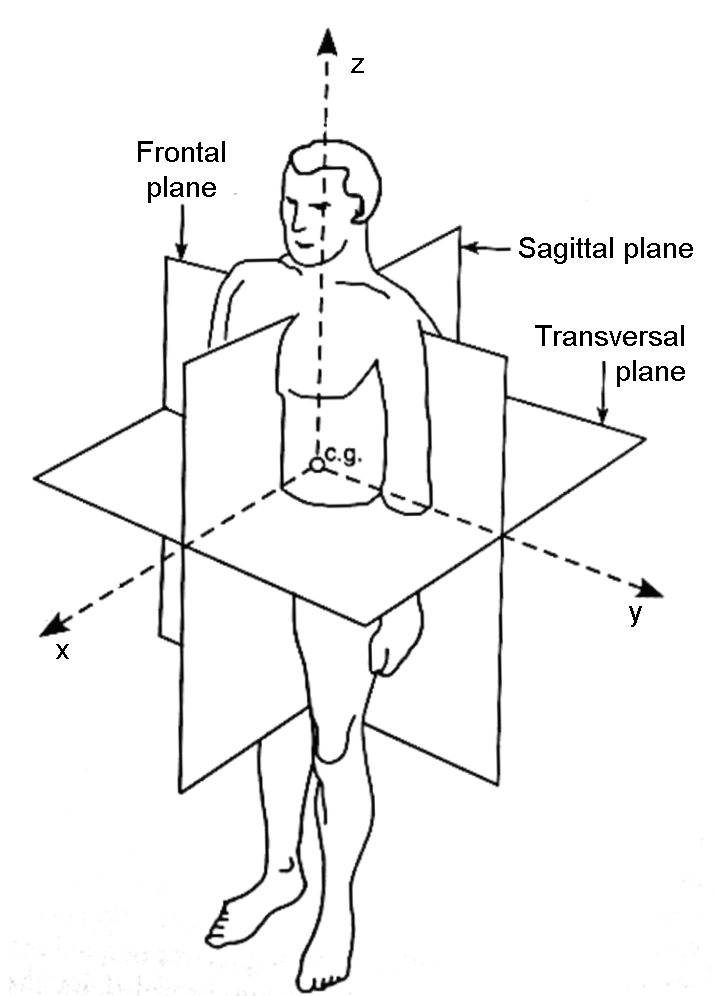
\includegraphics[scale=0.45]{axes.png}
\caption{Axes division of human body.}
\label{fig:axes}
\end{figure}

The basic characteristic of bipedal locomotion is the permanent change of the situation when the mechanism is supported by one foot (single support phase) and when both feet are in contact with the ground (double support phase). The second situation is statically stable and there are no additional moments affecting the robot. In terms of balance, the first situation is statically unstable because when one foot is on the ground, the other is transferred from the back to the front position producing lateral accelerations affecting the mechanism and all the weight remains in only one support foot. Thus, the locomotion mechanism changes its structure during a single walking cycle from an open to a closed kinematics chain. Each of these two cases present different dynamical situations and should be taken into account in artificial gait synthesis and control.

Robot walking, as humans, is performed in a three phase cycle (Figure \ref{fig:caminata}). The cycle is divided in two, left and right steps. At the begining, the humanoid is in a stable position with both feet on the ground (Figure \ref{fig:caminata} (a)) and all the body weight is transferred form one foot to the other. Then the step generation starts when the right foot leaves the ground in the swinging phase (Figure \ref{fig:caminata} (b), (c) and (d)). After the right foot touches the ground, the next (right) step with the same basic phases is started, and the whole cycle ends (Figure \ref{fig:caminata} (e)).

Swinging phase has also three sub-phases: acceleration, swinging and deceleration (Fig. \ref{fig:caminata} (b), (c) y (d), respectively). The acceleration phase takes its name due to the acceleration of the lifting leg that stops being supported in the ground and gives the impulse to the step. Once the support leg is overtaken, the lifting leg starts the swinging pahse in order to reach the ground with its consequent deceleration.

\begin{figure}[!hbt]
\centering
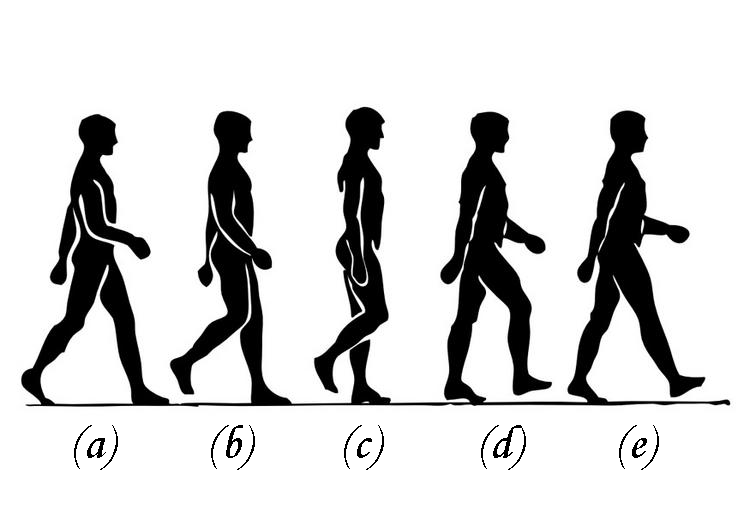
\includegraphics[scale=0.3]{Caminata}
\caption{Phases of biped walking.}
\label{fig:caminata}
\end{figure}

As in the case of the legs, the same occurs with the feet, what adds complexity to control the walking cycle. During a gait, a human foot has four different phases as one can see in Fig. \ref{fig:caminata_pie}. In (a) it is shown how the body weight is supported when the heel is touching the ground. In (b), the foot remains totally plane. In (c), the heel lifts and the weight goes to the front part of the foot. Finally, in (d) the foot is not in contact with the ground and it starts to swing.

\begin{figure}[!hbt]
\centering
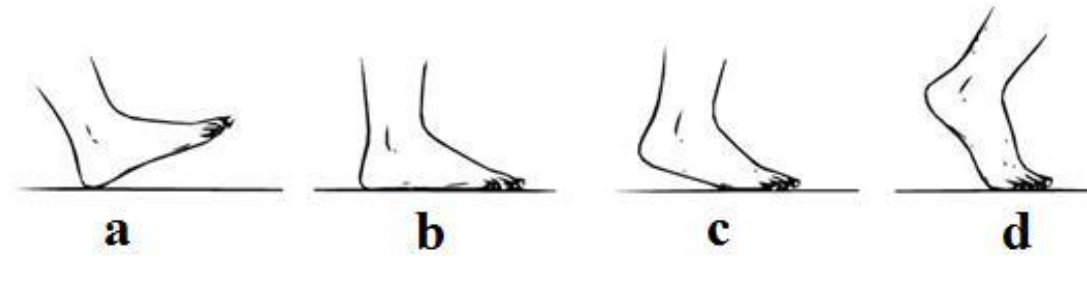
\includegraphics[scale=0.3]{caminata_pie.png}
\caption{Phases of foot support during a walk.}
\label{fig:caminata_pie}
\end{figure}

Almost all humanoid robots do not have articulated feet, due to the high complexity. They use plane and rigid feet and the control is done in the ankle joint. Some of them, as robot HRP-4 \cite{Kan}, have a joint called "active toe joint" which allows the movement of the toes. The reason of this improvement is related to reach a more natural and fluent walking.

However, in order to perform a stable walk, is not only necessary the lower body movement. The upper body is also involved in recovery movements. In an example, if a person stumbles. Unwittingly, he or she would move the opposite arm of the unbalanced leg, or even more, moving the torso in order to not to fall down. In the case of a biped robot, the same strategy is followed, what means a high increase of complexity in the robot stability control.

\section{Biped balance/equilibrium}
It is important for humanoid locomotion to avoid overturning during the walking or even to reach an upright position of its body. To prevent falling down, a necessary and suficient condicion is to ensure that there exists a contact area between the foot and the ground and not a line or a point \cite{Vuk2007}. Given a rectangular-shaped foot, the support area of the robot will be a polygon. In case that only on foot is touching the ground (single-support), the support area is the contact region between the sole and the ground, i.e., the footprint (Fig. 2.3(a)). On the contrary, when both feet are touching the ground (double-support), the support area will be determined by the footprints and the common tangents between them (Fig. 2.3(b)). It means that in double-support phase of the walk, the support area is bigger than in single-support phase, so stability is higher.

\begin{figure}[!hbt]
\centering
\subfigure[Single-support]{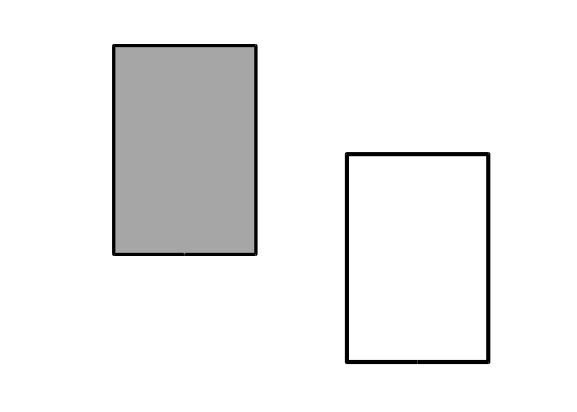
\includegraphics[scale=0.3]{apoyo_simple.png}}
\hspace{10mm}
\subfigure[Double-support]{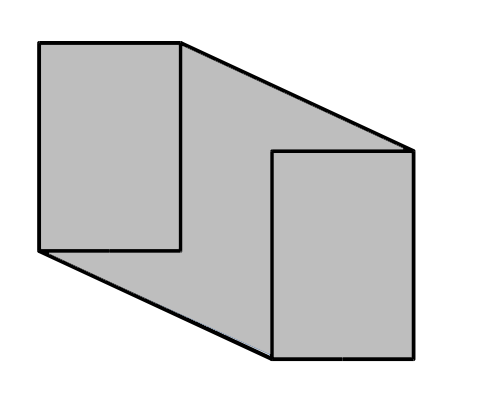
\includegraphics[scale=0.3]{apoyo_doble.png}}
\caption{Support areas depending on the support type.}
\label{fig:apoyo}
\end{figure}


\section{Zero Moment Point (ZMP)}
In \cite{Vuk2007}, Vukobratović makes a distinction between the term ``balance" used in the sense of maintaining an upright posture, and ``equilibrium", taking into account the D'Alembert's principle. The D'Alembert's principle states that the resultant of the external forces and the kinetic reaction acting on a body equals zero (condition of kinetic equilibrium). When the humanoid is falling since it is rotating about one foot edge, the D’Alembert’s principle still holds for a point on the foot edge where the pressure force acts. Anyway, this case cannot be contemplated as balanced in the sense of the definition previously provided. This point is called \textit{Center of Pressure (CoP)} and it is known as the point, in a single-support phase, where the pressure forces (normal to the sole) are equivalent to a single resultant force exerted at the point where the resultant moment is zero.

From the concept of the CoP, appears a new term known as \textit{Zero-Moment Point (ZMP)}. The ZMP is a point inside the support area where, always, the resulting dynamic reaction of the biped system is acting. In a more specific definition, the ZMP is a point inside the support area where the resultant of all forces and torques acting on the full body, is equal to zero.

Vukobratović \cite{Vuk2007} explains the difference between the CoP and ZMP: CoP and ZMP coincide only when both are inside the support area. When the ZMP goes to the edge of the support area, the humanoid body looses balance and it will fall down. In that case, the ZMP has no sense existing even the CoP.

Goswami presented that, mathematically was possible that the point could be outside of the support area and continue satisfying the equilibrium conditions \cite{Gos}. This point, called \textit{Foot Rotation Indicator (FRI)}, is defined as the point on the contact area between the ground and the foot, inside or outside the suppor area, where the resultant moment of the forces and torques applied on the foot are normal to the surface. Forces and torques applied mean the forces and torques at the ankle joint, and also other external forces, the foot wheight and reaction forces between the foot and the ground. 

However, Vukobratović, held that the ZMP can only exist inside the support area of the robot. When the ZMP comes close to the edge, any force or moment applied to the system, will produce a rotation about the foot edge and the robot will fall down. In this case, the reaction force of the ground will be at the foot edge and, therefore, it can not be considered as ZMP because there is no stability ensured. That is why the author suggests to denote the point as \textit{Fictitious ZMP} o \textit{FZMP}, if it is outside the support area. 
 
When the robot walking is enough slow to consider almost static, appears the term \textit{pseudo-ZMP}, which is the proyection over the ground of the \textit{Center of Gravity (CoG)} of the system. In such case, lateral accerlerations are so small and can be omitted and the \textit{pseudo-ZMP} = ZMP. Although the \textit{pseudo-ZMP} do not give precise information about the balance of the mecanism, it can be used in order to make a first aproximation in control and design of a humanoid robot.



\subsection{Equations of ZMP}
Let us consider the locomotion mechanism in the single-support phase, with the whole foot in contact with the ground (Fig. \ref{fig:pie} (a)). To simplify the analysis we can neglect the part of the mechanism above the ankle of the support foot (point A) and replace its influence by the force $F_A$ and moment $M_A$, whereby the weight of the foot itself acts at its gravity center (point G). The foot also experiences the ground reaction at point P, whose action keeps the whole mechanism in equilibrium.

\begin{figure}[!hbt]
\centering
\subfigure[]{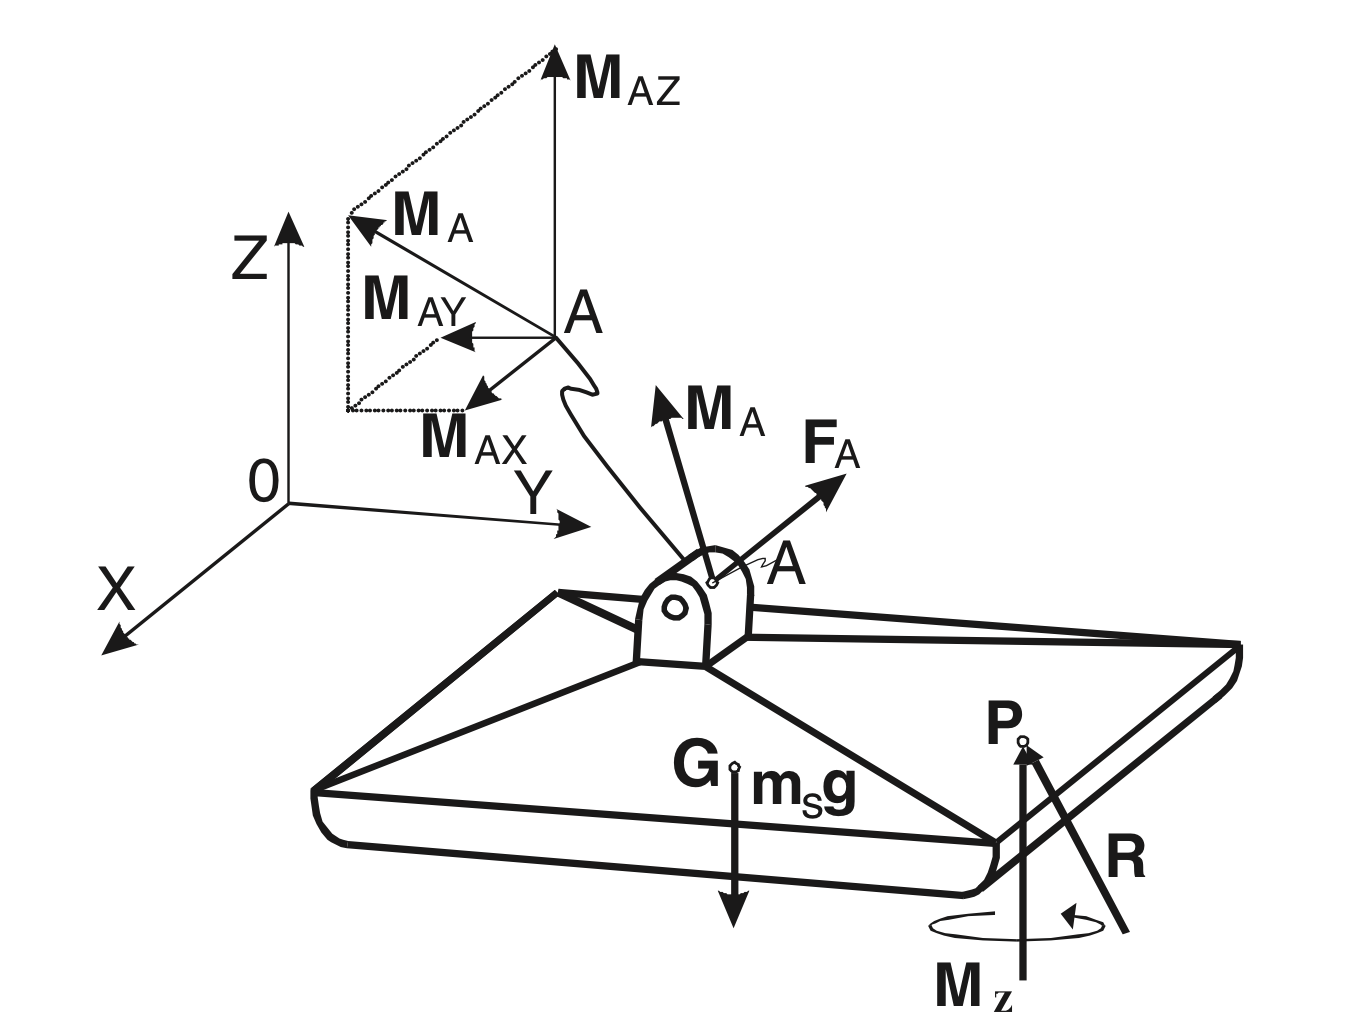
\includegraphics[scale=0.4]{pie.png}}
\subfigure[]{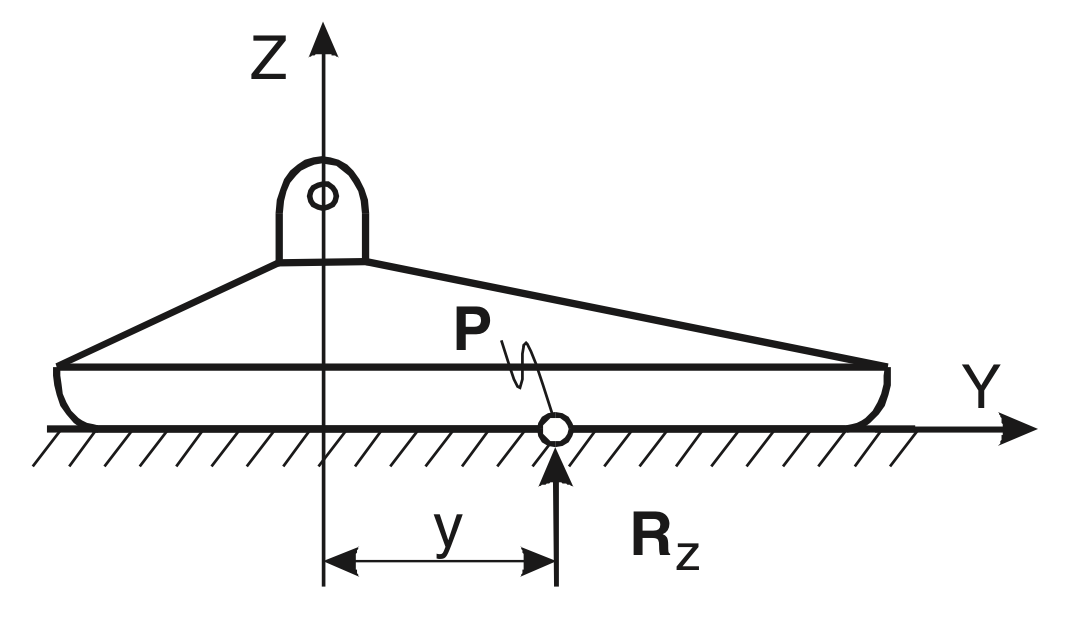
\includegraphics[scale=0.4]{pieYOZ.png}}
\caption{Forces acting on the foot of the bipedal mecanism \protect\cite{Vuk2004} }
\label{fig:pie}
\end{figure}

In general, the total ground reaction consists of three components of the force $R (R_x, R_y, R_z)$ and moment $M (M_x, M_y, M_z)$ exerted at the foot-ground contact point. During the support phase, it is assumed there is no shifting in the contact point, which means that horizontal reaction force $R_x$ and $R_y$ balances the horizontal component of the force $F_A$, whereas the vertical reaction moment $M_z$ represents the moment of friction reaction forces that balances the vertical component of the moment $M_A$ and the moment induced by the force $F_A$.

However, due to an unidirectional nature of the connection between the foot and the ground (it is obvious that the ground reaction force induced by foot action is always oriented upwards) horizontal components of all active moments ($M_A$) can be compensated for only by changing position of the reaction force $R$ within the support polygon. This is illustrated in Figure \ref{fig:pie} (b) where a planar case in $y-z$ plane is represented.

The moment $M_{Ax}$ is balanced by shifting the acting point of the force $R_z$, whose intensity is determined from the equation of balance of all the forces acting on the foot, by the corresponding distance $y$. It is necessary to emphasize that all the time the reaction force is within the area covered by the foot, the increase in the ankle moment will be compensated for by changing the position of this force $R_z$, and no horizontal components of the moments $M_x$ and $M_z$ will exist. This is the reason why in Figure \ref{fig:pie} at point $P$ only the $M_z$ component exists.

However, if the real support polygon is not large enough to encompass the appropriate position of the force $R$ to balance the action of external moments, the force $R$ will act at the foot edge and the uncompensated part of the horizontal component of the reaction moment will cause the mechanism’s rotation about the foot edge, which can result in the mechanism’s overturning. Therefore, it can said that the necessary and sufficient condition for the locomotion mechanism to be in dynamic equilibrium is that for the point $P$ on the sole where the ground reaction force is acting,

\begin{align}
M_x = 0, \nonumber \\
M_y = 0.
\end{align}

That is why the \textit{Zero-Moment Point} is called the contact point with the ground ($P$) where there no exist shifting, i.e., moments $M_x$ y $M_y$ are zero.

From Figure \ref{fig:pie}, static equilibrium equations for the supporting foot are obtained:
\begin{equation}
\sum \overrightarrow{F} = 0 \Rightarrow \overrightarrow{R} + \overrightarrow{F_A} + m_s g = 0
\label{eq:fuerzas}
\end{equation}
\begin{equation}
\sum \overrightarrow{M_O} = 0 \Rightarrow \overrightarrow{OP} \times \overrightarrow{R} + \overrightarrow{OG} \times m_sg + M_A + M_z + \overrightarrow{OA} \times F_A = 0,
\label{eq:momentos}
\end{equation}

where $\overrightarrow{OP}$, $\overrightarrow{OG}$ and $\overrightarrow{OA}$ are radius vectors from the origin of the coordinate system $O_{xyz}$ to the ground reaction force acting point ($P$), foot mass center ($G$), and ankle joint ($A$), respectively, while the foot mass is $m_s$. If we place the origin of the coordinate system at the point $P$ and project Eq. \eqref{eq:momentos} onto the z-axis, then the vertical component of the ground reaction momentc (actually, it is the ground friction moment) will be

\begin{equation}
M_z = M_{fr} = -M_A^Z + (\overrightarrow{OA} \times F_A)^Z
\end{equation}

In a general case, this moment is different from zero and can be reduced to zero only by the appropriate dynamics of the overall mechanism. However, the projection of ecuation \eqref{eq:momentos} onto the horizontal plane gives:
\begin{equation}
(\overrightarrow{OP} \times \overrightarrow{R})^H + \overrightarrow{OG} \times m_sg + (M_A)^H + (\overrightarrow{OA} \times F_A)^H = 0,
\label{eq:momentos}
\end{equation}
This equation is a basis for computing the position of the ground reaction force acting point ($P$) which gives the ZMP position.


\subsection{Relation between COG and ZMP}
When a humanoid robot is in the single-support phase during a walking cycle, its dynamics can be represented by a linear inverted pendulum where all body mass is concentrated in the CoG connected to the supporting foot point by means of a massless leg \cite{Kaj2001}. The pendulum can increase or decrease its length, thus simulating the functioning of the ankle joint.

Now, let us consider that the inverted pendulum instead of only one contact point considered above, has a contact polygon as the surface in contact with the ground (Figure \ref{fig:3DLIPM}).

\begin{figure}[!hbt]
\centering
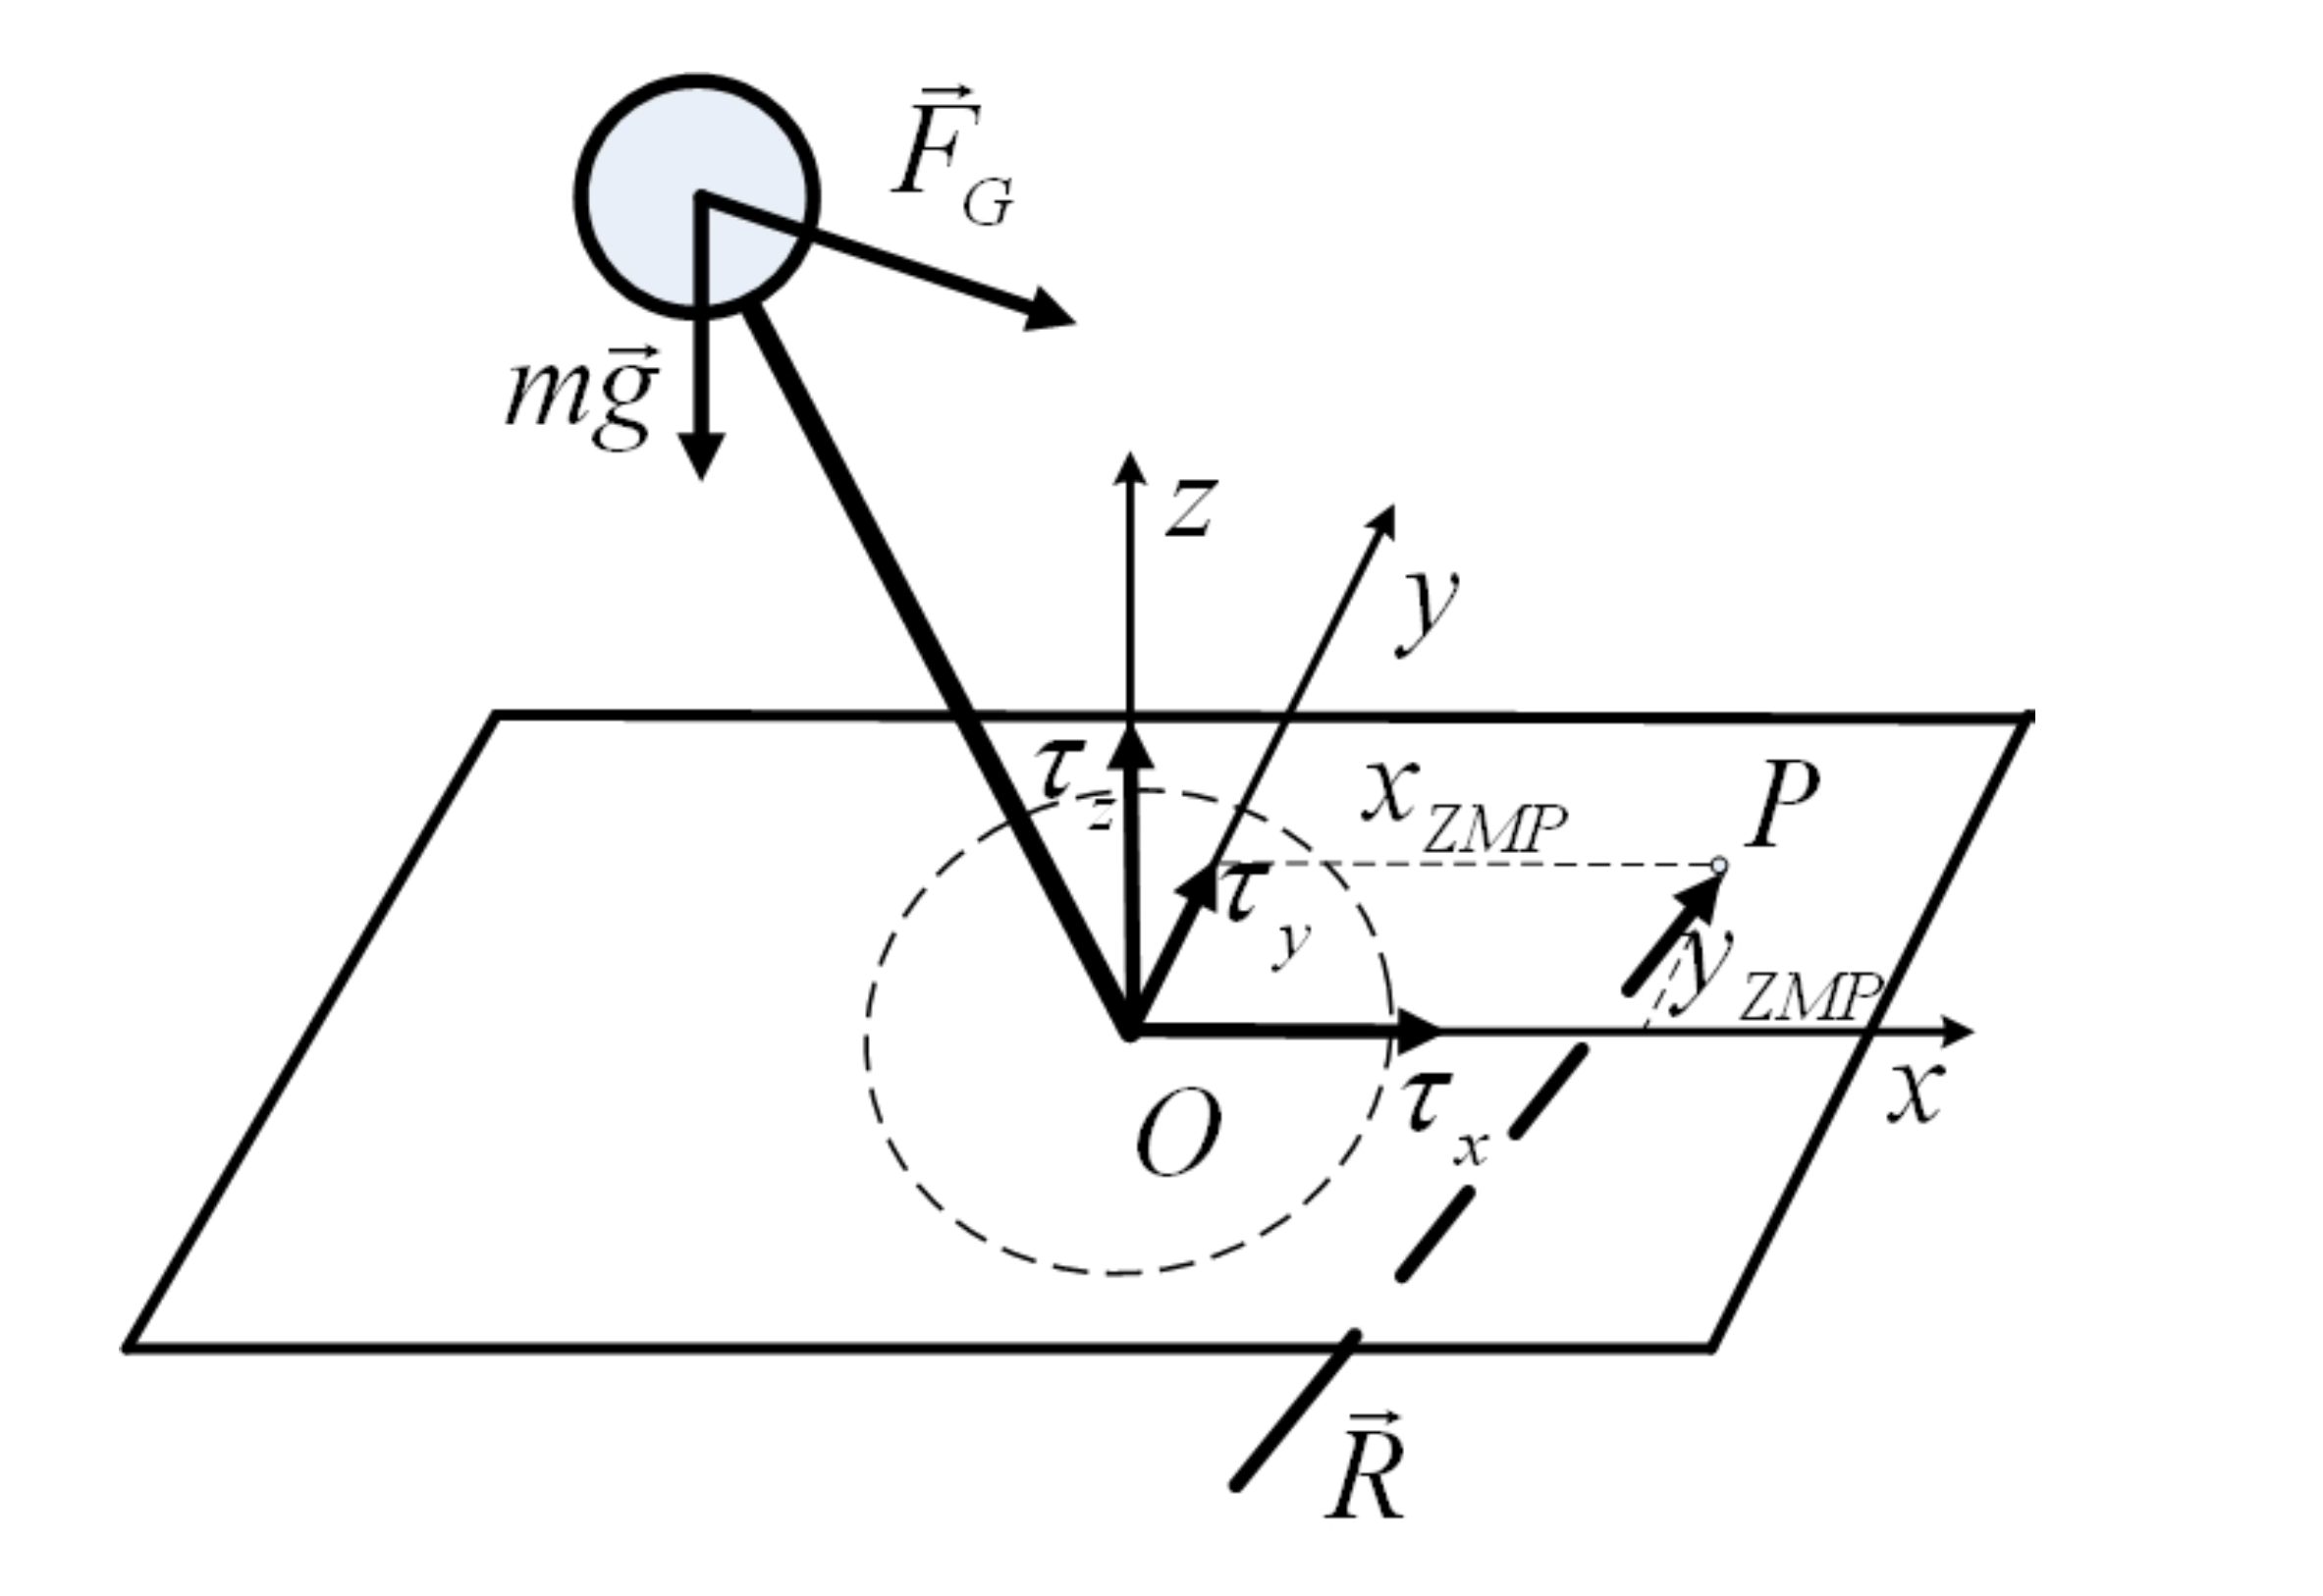
\includegraphics[scale=0.2]{3DLIPM.png}
\caption{3D Linear Inverted Pendulum with a contact polygon. \textcolor{red}{CITA}}
\label{fig:3DLIPM}
\end{figure}

Inertial $\overrightarrow{F_G}$ and gravity $m\overrightarrow{g}$ froces act on the point mass located in the COG of the humanoid robot. The contact of the pendulum with the ground produces a reaction force $\overrightarrow{R}$ and reaction moment $\overrightarrow{M_P}$ at point $P$ For any other point of the support polygon (taking point 0 as origin), the moment $M_0=[\tau_x, \tau_y, \tau_z]^T$ produced by the ground reaction force $\overrightarrow{R}$ is represented: 
\begin{equation}
M_0 = M_P + \overrightarrow{0P} \times \overrightarrow{R}
\label{eq:M0}
\end{equation}

If it is considered point P to be the ZMP of the system, then from the interpretation of the ZMP presented above $M_P = 0$. In this case we can denote vector $\overrightarrow{OP} = [x_{ZMP}, y_{ZMP}, z_{ZMP}]^T$ and eq. \eqref{eq:M0} gives the following equation:
\begin{equation}
\begin{pmatrix}
\tau_x \\
\tau_y \\
\tau_z 
\end{pmatrix} 
=
\begin{pmatrix}
x_{ZMP} \\
y_{ZMP} \\
z_{ZMP}
\end{pmatrix}
\times \overrightarrow{R}
\label{eq:1}
\end{equation}

From the other side, applying Newton’s law of mechanics to system in Figure \ref{fig:3DLIPM}:
\begin{equation}
m \overrightarrow{a_G} = \overrightarrow{R} - m\overrightarrow{g}
\label{eq:newton}
\end{equation}

where $\overrightarrow{a_G} = [\ddot{x}, \ddot{y}, \ddot{z}]^T$ is the acceleration of the COG. From equation \eqref{eq:newton} it is obtained:
\begin{equation}
\overrightarrow{R} = m 
\begin{pmatrix}
\ddot{x} \\
\ddot{y} \\
\ddot{z} + g
\end{pmatrix}
\label{eq:2}
\end{equation}

Substituting equation \eqref{eq:2} into the equation of balance of moments \eqref{eq:1} it is obtained:
\begin{equation}
\begin{pmatrix}
\tau_x \\
\tau_y \\
\tau_z 
\end{pmatrix} 
= m
\begin{pmatrix}
x_{ZMP} \\
y_{ZMP} \\
z_{ZMP}
\end{pmatrix}
\times
\begin{pmatrix}
\ddot{x} \\
\ddot{y} \\
\ddot{z} + g
\end{pmatrix}
\end{equation}

After a cross product and taking into account that $z_{zmp} = 0$, because the ZMP lies into the ground:
\begin{equation}
\begin{pmatrix}
\tau_x \\
\tau_y \\
\tau_z 
\end{pmatrix} 
= m
\begin{pmatrix}
y_{ZMP}(\ddot{z}+g) \\
-x_{ZMP}(\ddot{z}+g) \\
x_{ZMP}\ddot{y}-y_{ZMP}\ddot{x}
\end{pmatrix}
\label{eq:3}
\end{equation}

From \eqref{eq:3}, it can be stated the ZMP position of the system:
\begin{equation}
x_{ZMP} = -\frac{\tau_y}{m(\ddot{z}+g)}
\label{eq:x}
\end{equation}
\begin{equation}
y_{ZMP} = \frac{\tau_x}{m(\ddot{z}+g)}
\label{eq:y}
\end{equation}

If it is supposed that the COG always remains within the horizontal plain intersecting the $z$ axis in the point $z_c$ (one of the constraints of the 3D-LIPM model), then the vertical component of the COG acceleration $\ddot{z}=0$. Then, finally, equations \eqref{eq:x} and \eqref{eq:y} are:
\begin{equation}
x_{ZMP} = -\frac{\tau_y}{mg}
\label{eq:xzmp}
\end{equation}
\begin{equation}
y_{ZMP} = \frac{\tau_x}{mg}
\label{eq:yzmp}
\end{equation}

When the ankle joint is displaced from the ground as in Figure \textcolor{red}{FIGURE}, ZMP equations take the form:

\begin{equation}
x_{ZMP} = -\frac{\tau_y+hF_x}{mg}
\label{eq:xzmp}
\end{equation}
\begin{equation}
y_{ZMP} = \frac{\tau_x+hFy}{mg}
\label{eq:yzmp}
\end{equation}

where $h$ is the distance between the ground and the measuring point, i.e, the height of the sole. 
These are the \textit{ZMP equations}, without forgetting it was considered before that lateral accelerations of the COG $\ddot{x}=0$ and $\ddot{y}=0$. One can see that moments $\tau_x$ and $\tau_y$ in $x$ and $y$ directions respectively affect the ZMP position of the mecanism and it can loose balance because of their change.

If we take into account these lateral accelerations of the COG, the ZMP can be expressed as a function of the acceleration of the COG as: \textcolor{red}{REFERENCIA?}
\begin{equation}
x_{ZMP}=x_{COG}-\frac{z_c}{g}\ddot{x}_{COG}
\end{equation}
\begin{equation}
y_{ZMP}=y_{COG}-\frac{z_c}{g}\ddot{y}_{COG}
\end{equation}

These equations can only be applied to compute ZMP in single-support phase. In the case of the double-support phase, it is necessary to calculate the weighted average of the sensor measurements form both feet as recommended in \cite[pp. 82-83]{Kaj2005}. Therefore, the resulting equations for ZMP in double-support phase are:

\begin{equation}
x_{ZMP} = -\frac{x_{ZMP}^{R} \cdot F_{z}^{R} + x_{ZMP}^{L} \cdot F_{y}^{L}}{F_{z}^{R}+F_{z}^{L}}
\end{equation}
\begin{equation}
y_{ZMP} = \frac{y_{ZMP}^{R} \cdot F_{z}^{R} + y_{ZMP}^{L} \cdot F_{z}^{L}}{F_{z}^{R}+F_{z}^{L}}
\end{equation}
where the upper index $R$ represents the right foot and $L$ the left one.

\subsection{ZMP areas.}
As mentioned before, ZMP is a point in the sole which depends on the forces and moments applied to the robot. Therefore, depending on the magnitude of that forces, ZMP will change and it becomes a dynamic parameter. As suggested in \cite{Vuk2007}, three regions are defined depending on the position of the ZMP as one can see in Fig. \ref{fig:zonas}.
In the balanced area (safe region), the control action will not actuate. In the nearly critical region, the control action will actuate as a secondary solution. This may be the case of a walking task. As humans do, the robot may use its arms in order to reduce the zero-moment point position closer to the safe region. Finally, in the critical region, the stabilizer will actually disconnect the ongoing task and actuate on the full body. Even if this region is still stable, the balance may be easily lost. 


\begin{figure}[!hbt]
\centering
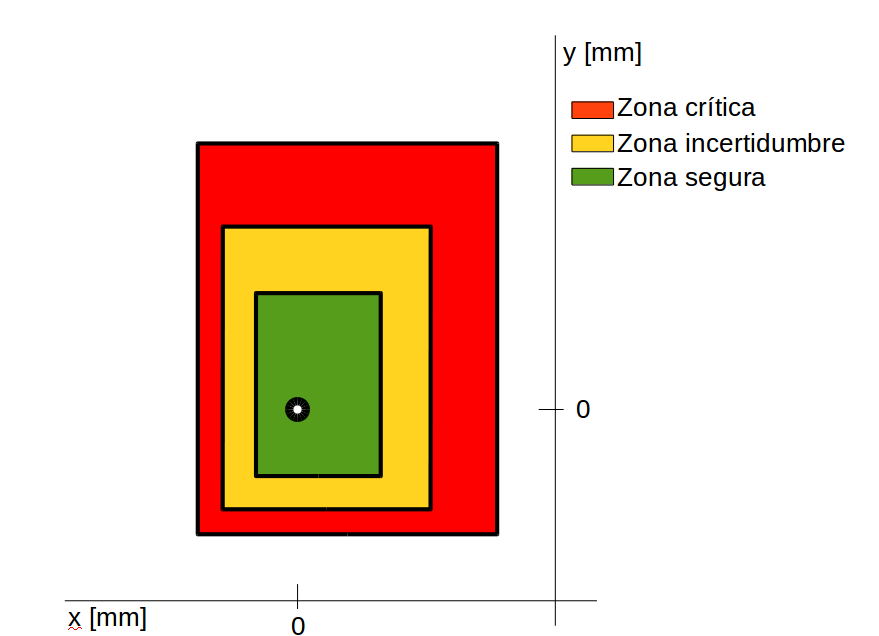
\includegraphics[scale=0.3]{zonas}
\caption{ZMP stability regions in single-support.}
\label{fig:zonas}
\end{figure}



\section{Biped modeling}
Humanoid robots have a very complex dynamics because of their complex mechanical configuration and they require a high computational cost. Figure ??? represents a simplified mechanical configuration of a typical humanoid robot. As one can see, the high number of DOFs due to the precise knowledge of robot dynamics including, mass, location of the centre of mass and moments of inertia of each link, make stable biped locomotion very complex. Thus, different simplified models of the mechanics have been developed. These methods use limited knowledge of the dynamics and the humanoid is usually represented by a planar inverted pendulum with the base representing the ankle joint and, in case of 3D locomotion, the Three-Dimensional Inverted Pendulum Mode (3D-LIPM) \cite{Kaj2001}.

\graphicspath{{03_plataforma/Imagenes/}}

\chapter{Platform description} 
\label{cap:platform_description}
\section{Humanoid robot TEO}
Humanoid robot RH-2, also known as TEO (Task Environment Operator), from University Carlos III of Madrid, is and advanced version of humanoid robots RH-0 and RH-1. TEO is 165 cm high overtaking 150 cm of RH-1 and 120 cm of RH-0. It wheights about 60 kg and it can carry about 2 kg of payload. It has 26 DOFs (28 DOFs taking into account head motors), more DOFs than in previous versions. In Figure \ref{fig:gdl} one can see the robot DOFs, besides their direction of rotaton, being 6 DOFs for each leg, 6 DOFs for each arm, 2 DOFs for the torso and 2 DOFs for the head.

\begin{figure}[!hbt]
\centering
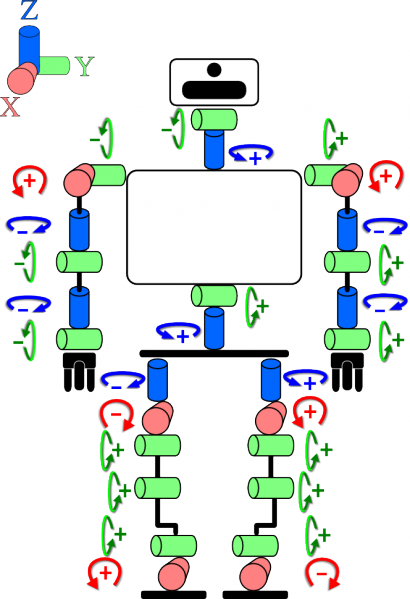
\includegraphics[scale=0.45]{teo_gdl.png}
\caption{Distribución de grados de libertad del robot TEO.}
\label{fig:gdl}
\end{figure}

The robot has 4 microprocessors: locomotion, manipulation, artificial vision tasks and last, the main processor which manages the others. The locomotion processor, that controls the legs and the torso, will be responsible for getting the sensors information and maintain the robot in a balance and upright position, being static or in a walking cycle. The manipulation processor controls the movement of the arms and the head. The processor responsible for the computer vision uses a camera with infrarred sensor ASUS located in the head.

The communication system is based on the CAN-bus protocol. Making a sagittal and transversal division, there are 4 CAN-bus lines: 1 line per each arm and neck, and 1 line per each leg and torso.

For data acquisition, the robot has a inertial sensor located at the trunk and Force-Torque sensors located at the robot ankles and wrists. F-T sensors are plugged into real time data acquisition PCI cards. Including F-T sensors is an important difference and advantage respect RH-2 predecessors. They allow to close the control loop and then, to obtain a kind of feedback which is necessary to accomplish tasks successfully.

The Control level is divided into 2 layers. At joint level, each servo not only closes the servo loop, it also synchronizes with other devices and absolute encoders provide a feedback of joint motors. At task-oriented control level, high level executions are done. This layer is directly connected with the joint level control. Examples of appliance are manipulation of objects or stability control which is the aim of this project. Figure \ref{fig:comms} shows the general communication diagram.

\begin{figure}[!hbt]
\centering
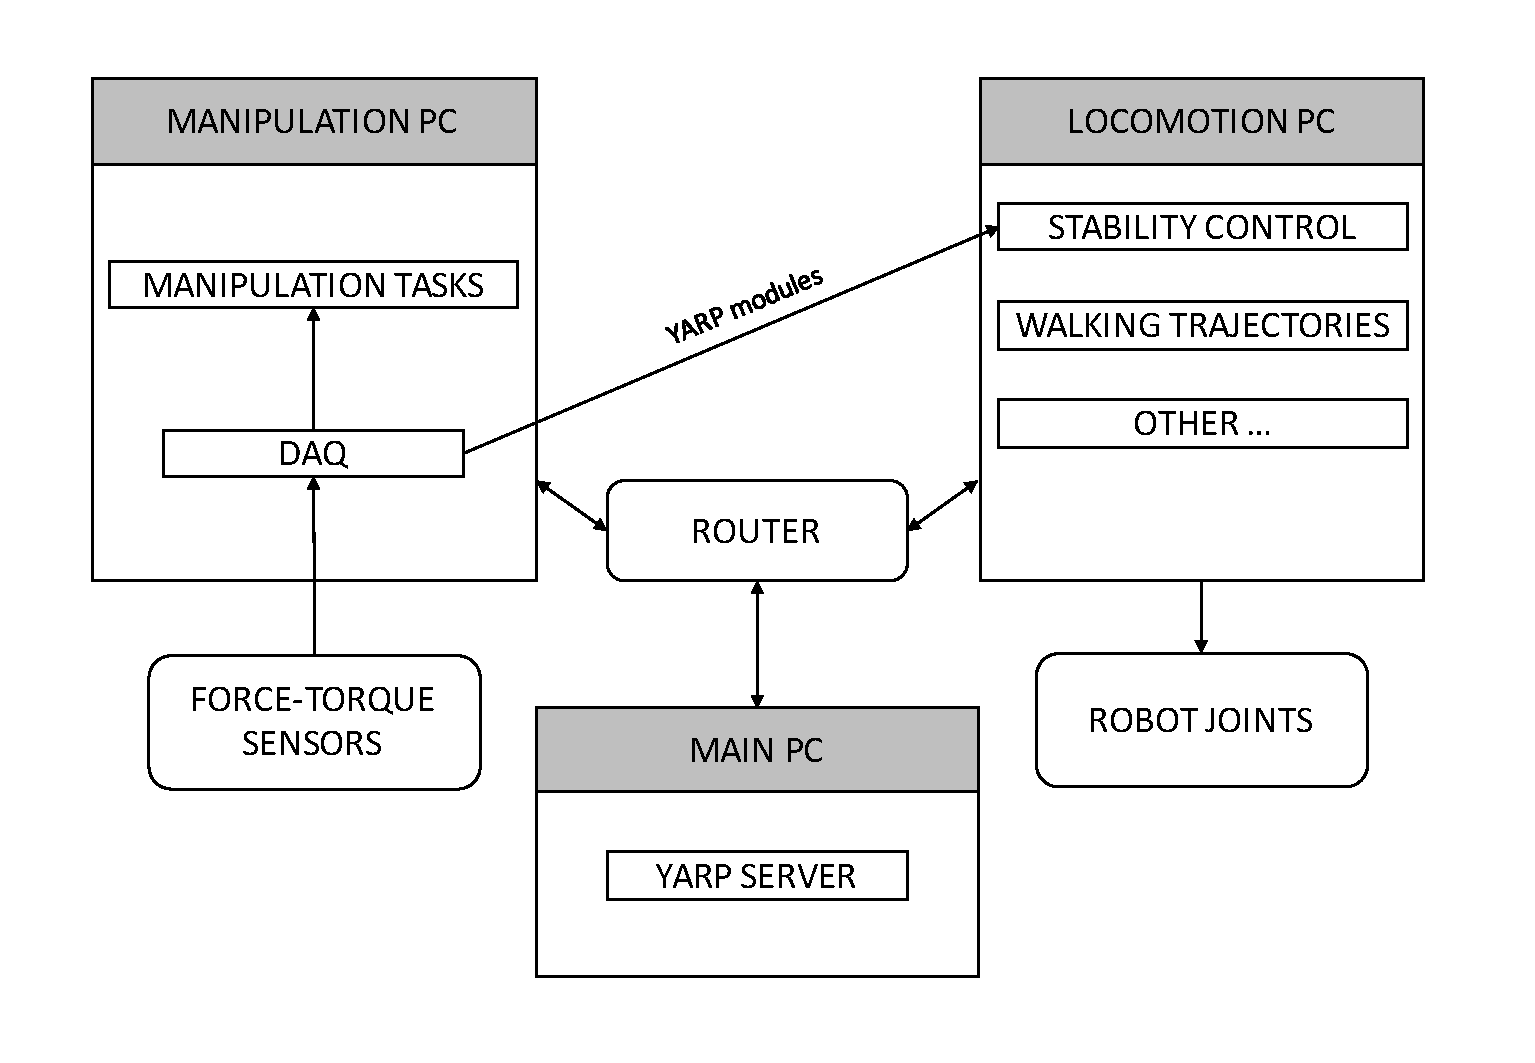
\includegraphics[scale=0.5]{comms.pdf}
\label{fig:comms}
\caption{Basic communications diagram}
\end{figure}

\section{Force/Torque sensors}
Force-Torque (F-T) sensors are based on strain gauge sensors arranged in such a way that allows to obtain force and moment measures in all axes of the 3D space. 

The sensors used in the platform, are the commercial JR3 F-T sensors described in Table\ref{table:sensores}. Look at the full scales difference between the sensors used in the wrists joints and the ones used in the ankle joints. Ankle sensors must be able to support greater forces and moments including the ones exerted by the own robot.

\begin{table}[!hbt]
\centering
\begin{tabular}{|c|c|c|c|c|}
\hline
Joint & Model & $F_{x,y}$ & $F_z$ & $M_{x,y,z}$\\
\hline
Wrist & 50M31A & 100N & 200N & 5 Nm\\ 
\hline
Ankle & 85M35A & 250N & 500N & 212Nm\\
\hline
\end{tabular}
\caption{F-T sensor models and characteristics. [JR3 Inc.]}
\label{table:sensores}
\end{table}

According to the manufacturer, the two first digits of the model show the sensor diameter, followed by the serie, and the next two digits, the thickness. As mentioned before, the ankle sensors are bigger and they support greater forces and moments. The sensors used in this Master Thesis are the ones mentioned in Table \ref{table:sensores} for ankle joints.

Serie M sensors include inner electronics in order to filter noise, digital output to use a data acquisition PCI card from the same manufacturer and an analogical output option. The nominal precission of all sensors of serie M is 1\% of full scale, and a 1/4000 full scale resolution.

The sensors used in this work, provide the option of acquiring data in International System Units or Imperial System Units, according to Figure \ref{fig:sensor}.

\begin{figure}[!hbt]
\centering
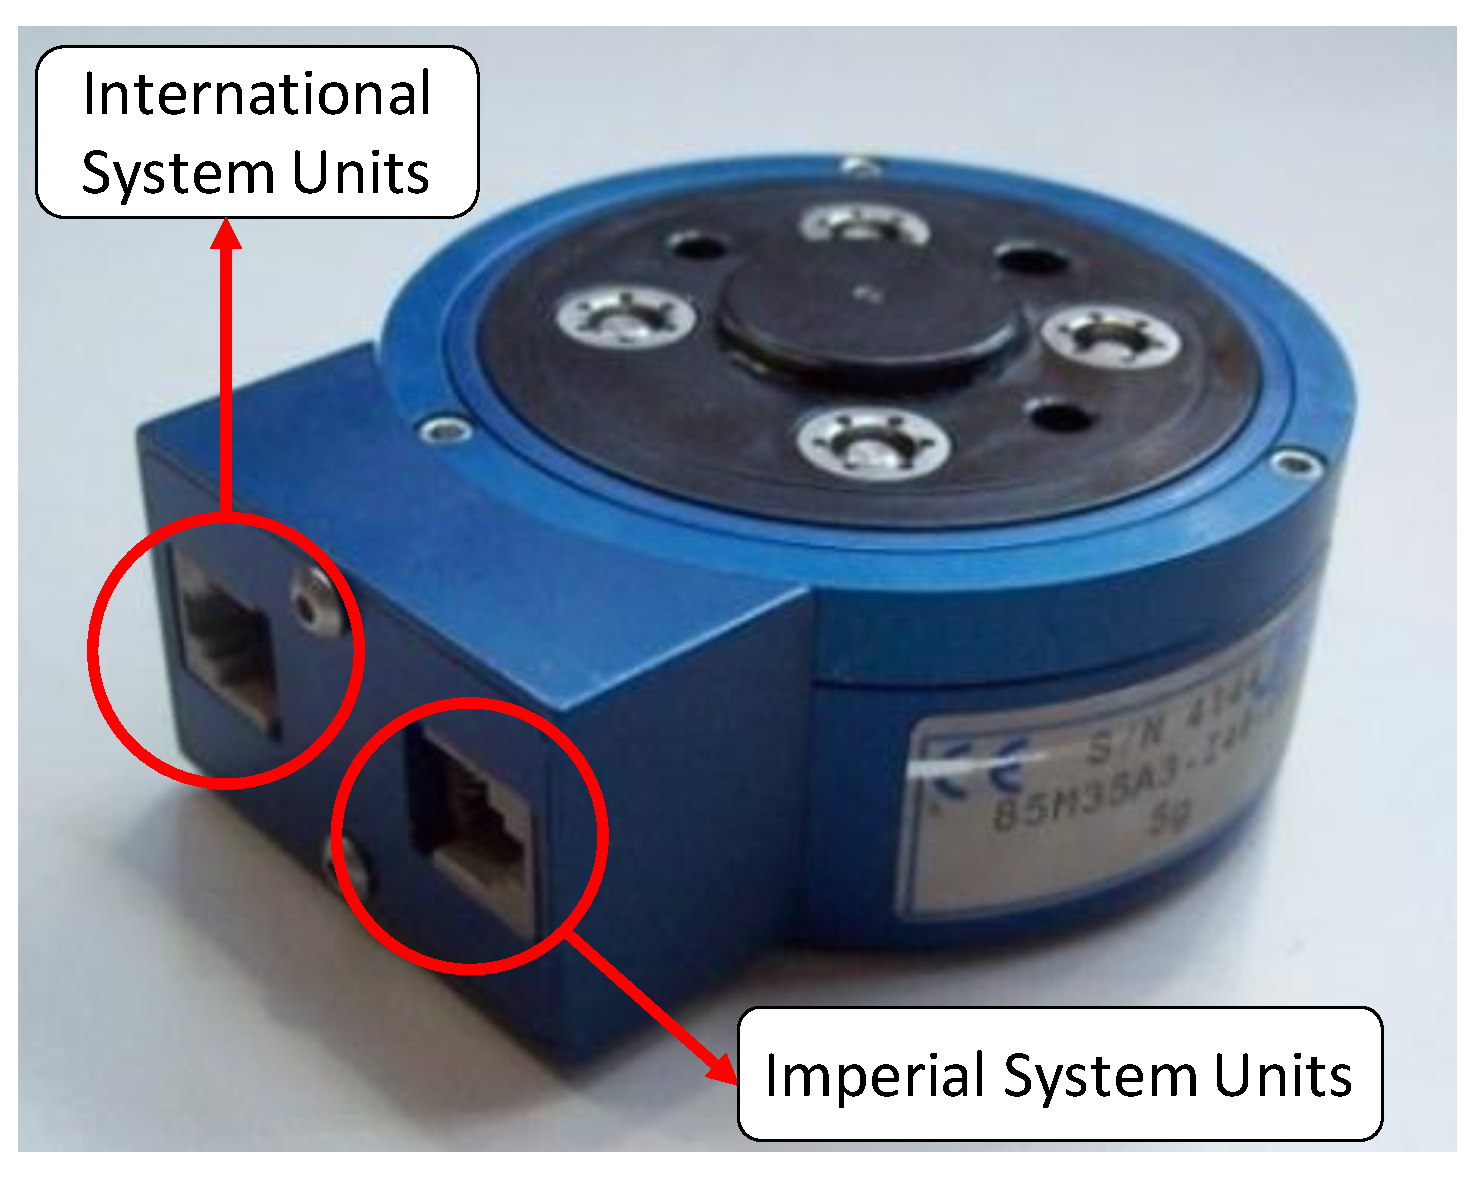
\includegraphics[scale=0.25]{sensor.pdf}
\label{fig:sensor}
\caption{JR3 model 85M35A Force-Torque sensor}
\end{figure}

\section{Data Acquisition}
The PCI cards used for data acquisition are PCI 1592D from JR3 Inc, which has 4 ports (named as in Figure ???). The sensors are plugged through a 6 or 8 pinout cables (RJ-11 and RJ-45, respectively). In the case of RJ-45, two pinouts are not used. The PCI card uses these cables to receive high speed data and provide power supply to the sensors. About the PCI supply, it is provided by the PCI slot form the computer where it is installed.

In order to access to received data from the sensors, it is necessary to access to card memory, specifying the memory address for each available data. These addresses can be found at [ANEXO. DATOS DEL FABRICANTE].

It is important to take into account that the forces and torques obtained from the sensors and processed by the card, are in the International System Units. Forces are given in Newton [N] and torques are given in tenths of a newton per meter [dN·m].

\subsection{Acquisition program}
The data acquisition of forces and moments form the sensors is done by user programs by means of the data aquisition card. 

The \textit{jr3pci2channelYarp} program (See ANEXOS) reads data from 2 Force/Torque Sensors with a rate of $40 \mu s$.

The sequence of the program is the following: reads data from sensors, scales the data to SI units, clusters the data into a YARP Bottle object and sends it through YARP ports.

\graphicspath{{04_control_architecture/Imagenes/}}
\chapter{Control Architecture}
\section{Introduction}
Vukobratovic \cite{Vuk1970} was one of the first researchers involved in the stability of bipedal robots, followed by \cite{Kaj2001} and \cite{Kim2004}. In all their studies, the biped robot was usually represented by a planar inverted pendulum with the base representing the foot and the ankle joint. And in the latest control strategies, researchers divide robot balance control into the hip strategy and the ankle strategy \textcolor{red}{REFERENCIA Y EXTENDER MÁS}. The basis of both stategies are close to the ZMP areas explained in previous sections. When the robot is in a stable posture and a disturbance is applied, depending the magnitude or the application point of that distrubance, the robot will react different. If the change of the ZMP position remains in a stable area, the control will react by the motion of the ankle joints to recover the robot balance. Nevertheless, if the ZMP position reaches an uncertain-stability area, it will be also necessary to move the hip joints to recover balance. Even a gait will be necessary if the loss of stability is unavoidable. 

A humanoid is an electromechanical system, so it should have all type of errors: structure flexion, small blacklash between motion parts, etc. Also it will operate in a co-existing environment with humans, so the disturbances are unexpected at any time. Therefore, the Stabilizer is an essential element to provide stable human-like walking of a humanoid robot. The Stabilizer should perform two basic operations:
\begin{itemize}
\item[1.] When the humanoid robot walks, it should correct the robot’s walking trajectory in order to provide the secure position at any time of its motion.
\item[2.] When the humanoid robot has stopped, it should control its posture.
\end{itemize}

Thus, the Stabilizer can be decoupled into ZMP and Attitude controllers. This Master Thesis will deal with the issue of maintaining an upright posture while the robot is in a static position, without following a motion pattern.


\section{Linear Inverted Pendulum Model}
The linear inverted pendulum is the most basic model used to simplify humanoids' body. The basis of the pendulum are a mass $m$ linked to a pivot point by means of a massless link of longitude $l$ as in Figure \ref{fig:pendulo_inv}.

The mass $m$ represents the total mass of the modelled system, a humanoid robot in this case, located at its Centre of Mass (CoM), and the longitude $l$ is the distance between the pivot point to the CoM. Its dynamical model in a planar, for example XZ case, is expressed by the equation \eqref{eq:pendulo}, if gravitational force is considered the only force acting in the system.

\begin{figure}
\centering
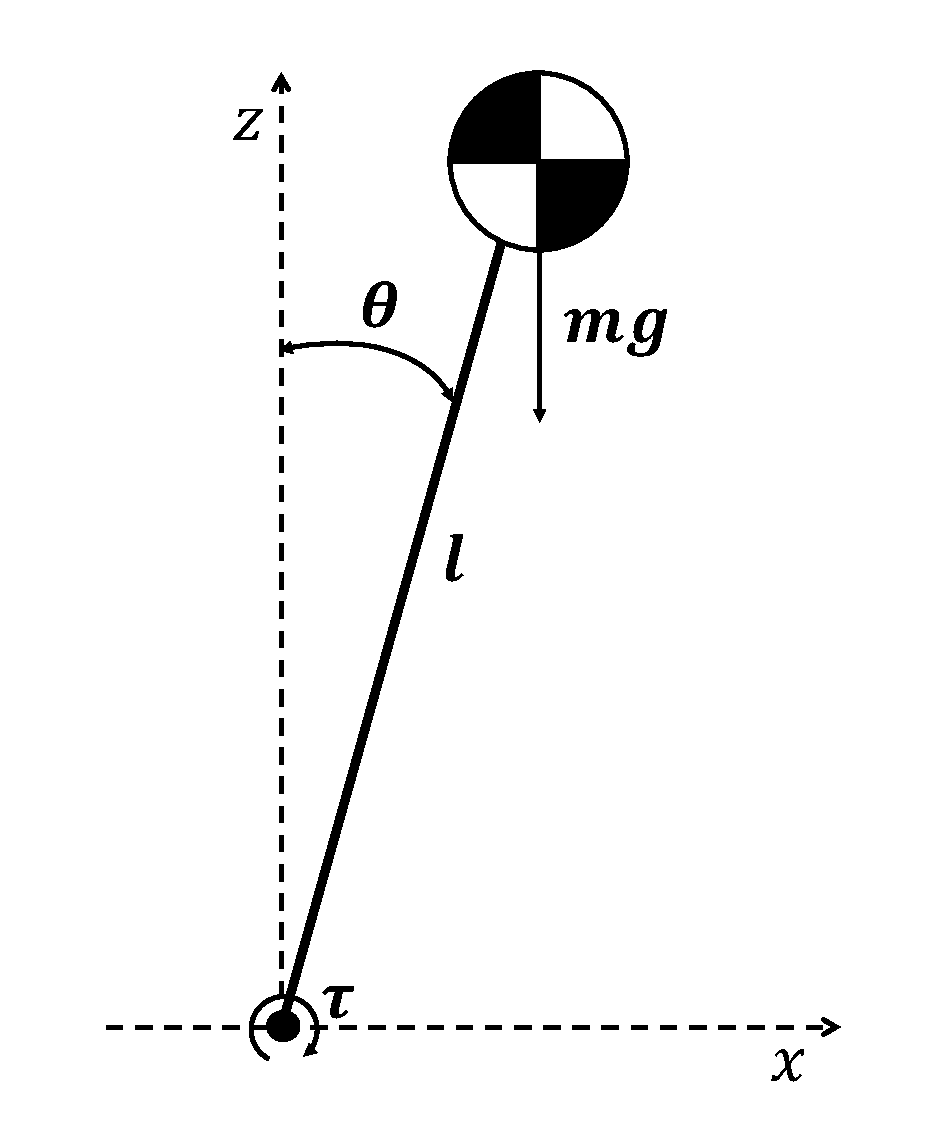
\includegraphics[scale=0.3]{penduloInv.pdf}
\caption{Single inverted pendulum.}
\label{fig:pendulo_inv}
\end{figure}

\begin{equation}
\tau_0 = ml^2 \ddot{\theta} - mgl\sin\theta
\label{eq:pendulo}
\end{equation}

where $\tau_0$ is the torque generated by the ankle joint, $\theta$ its angular position, $\ddot{\theta}$ its angular acceleration and $l$, the distance between the joint and the CoM. For simplification of a control task, let us make a linearization of nonlinear differential equations, taking the aproximation that perturbations are small enough to consider  $\sin\theta = \theta$. It is not defined how small these angles have to be in practice to apply the linearization assumptions, but in this case it is assume that $\theta \leq 10º$ Then, equation \eqref{eq:pendulo} changes to linearized equation \eqref{eq:pendulo2}
\begin{equation}
\tau_0 = ml^2 \ddot{\theta} - mgl\theta
\label{eq:pendulo2}
\end{equation}

The main complexity of this model is the fact that equation \eqref{eq:pendulo2} does not give the possibility of controlling the ZMP by angular position of the ankle joint. To overcome this problem, the inverted pendulum model can be slightly modified. The link of the pendulum which connects the ankle joint to the concentrated mass (CoM) is generally assumed to be rigid. However, in the real humanoid mechanism it is slightly flexible because the leg length is relatively long and the mechanical structure suffers form flexibility and small backlashes. Because of this compliance, the humanoid robot exhibits the characteristics of a lightly damped structure \cite{Kim2004}. For example, in a static case when the ankle joint is under position control, a pushing external force can easily excite an oscillation. This oscillation exists even when the position error in every joint is zero. This phenomenon is prevalent in the fast dynamical gait; therefore it is very imortant to implement a control mechanism allowing ZMP fast correction considering the stiffness of the humanoid robot links. The most suitable model in this case will be a single mass inverted pendulum with compliant joint as shown in Figure \ref{fig:pendulo_elast}, where $u$ denotes the ankle joint reference angle and $\theta$ denotes the actual inclined angle produced by the compliance of the mechanical structure of the humanoid, $k$ denotes the stiffness of the leg and $\tau_0$ is the torque produced by the motor of the ankle joint to place the inverted pendulum into the desired angular position. Then, the torque $\tau_0$ should be expressed as:

\begin{equation}
\tau_0 = k(\theta - u)
\label{eq:pendulo3}
\end{equation}

\begin{figure}
\centering
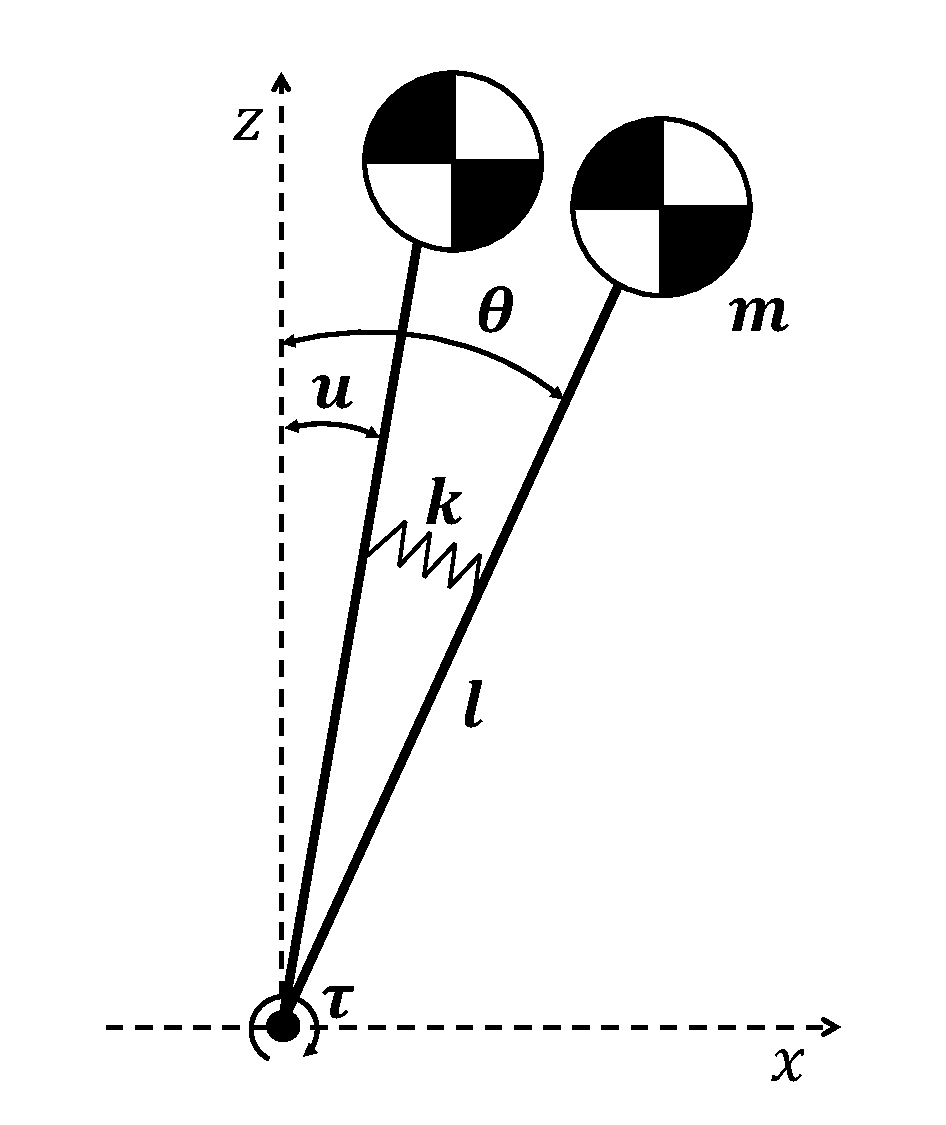
\includegraphics[scale=0.3]{penduloCompliant.pdf}
\caption{Single inverted pendulum with compliant joint.}
\label{fig:pendulo_elast}
\end{figure}

Taking the Laplace transform of equation \ref{eq:pendulo2}, it is obtained: 
\begin{equation}
T(s) = mgl\theta(s)- ml^2s^2\theta(s) 
\label{eq:par}
\end{equation}

The Laplace transform of equation \eqref{eq:pendulo3} is:
\begin{equation}
T(s) = k(\theta(s) - U(s))
\label{eq:par2}
\end{equation}

Clearing $\theta(s)$ from equation \eqref{eq:par2} and placing it into the equation \eqref{eq:par} and simplifying, the transfer function is obtained:
\begin{equation}
\frac{T(s)}{U(s)} = k \frac{-s^2+(\beta - \alpha)}{s^2 + \alpha}
\label{eq:TFpar}
\end{equation}

where:
\begin{equation}
\alpha = \frac{k-mgl}{ml^2}
\end{equation}
\begin{equation}
\beta = \frac{k}{ml^2}
\end{equation}

On the other hand, from equation \eqref{eq:xzmp} relating the moment produced by the ground reaction force around $y$ axis with $x$ ZMP direction (the planar XZ case of the inverted pendulum is considered) we can get:
\begin{equation}
\tau_y = -mgx_{ZMP} = - F_z x_{ZMP}
\label{eq:zmp}
\end{equation} 

and then the Laplace transform of the equation \eqref{eq:zmp} is:
\begin{equation}
\tau_y(s) = - F_z x_{ZMP}(s)
\label{eq:TFzmp}
\end{equation}

For the static equilibrium of the system, the moment generated y the motor of the ankle joint should compensate the moment produced by the ground reaction force:
\begin{equation}
\tau_0 = \tau_y
\end{equation}

The relation between $\tau_y$ and $x_{ZMP}$ is linear, therefore, placing \eqref{eq:TFzmp} into \eqref{eq:TFpar} we get the following transfer function relating ZMP to ankle joint position: 
\begin{equation}
\frac{x_{ZMP}(s)}{U(s)} = - k_1 \frac{-s^2+(\beta - \alpha)}{s^2 + \alpha}
\end{equation}

where $k_1 = \frac{k}{mg}$.

In equation \eqref{eq:TFpar} $x_{ZMP}(s)$ is the output and $U(s)$ is the input of the system.

The state space representation of the dynamical system in the standard form is:
\begin{equation}
\mathbf{\dot{x}} = \mathbf{A}\textbf{x} + \mathbf{B}u
\label{eq:ss1}
\end{equation}

\begin{equation}
y = \mathbf{C}\textbf{x} + Du
\label{eq:ss2}
\end{equation}

where $\mathbf{x}$ is a state ($n$-vector), $y$ is the output (escalar), $u$ - control (scalar), $\mathbf{A}$ - $n \times n$ constant  matrix, $\mathbf{B}$ - $n \times 1$ constant matrix, $\mathbf{C}$ - $1 \times n$ constant matrix and $D$ a scalar.

To obtain the state representation of the inverted pendulum system let us define state variables $x_1$ and $x_2$ by:
\begin{equation}
x_1 = \theta
\label{eq:x1}
\end{equation}
\begin{equation}
x_2 = \dot{x_1} = \dot{\theta}
\label{eq:x2}
\end{equation} 

where angle $\theta$ denotes the rotation of the pendulum about the ankle and $\dot{\theta}$ its angular velocity. We consider the ZMP as the output of the system, then $y = x_{ZMP}$ in the XZ planar case. From the definition of state space equations \eqref{eq:ss1} - \eqref{eq:x2} and the linearized equations of the inverted pendulum motions \eqref{eq:pendulo2} and \eqref{eq:pendulo3} we obtain the state space representation of the system:
\begin{equation}
\begin{bmatrix}
\dot{x_1} \\
\dot{x_2}
\end{bmatrix} 
= 
\begin{bmatrix}
0 & 1 \\
-\alpha & 0
\end{bmatrix}
\begin{bmatrix}
x_1 \\
x_2
\end{bmatrix}
+
\begin{bmatrix}
0 \\
1
\end{bmatrix}
u
\label{eq:state_space}
\end{equation}
\begin{equation}
y = \begin{bmatrix}
-k_1\beta & 0 
\end{bmatrix}
\begin{bmatrix}
x_1 \\
x_2
\end{bmatrix}
+ \begin{bmatrix}
k_1
\end{bmatrix}
u
\label{eq:state_space_out}
\end{equation}

\section{Feedback in state space. The Linear Quadratic Regulator}

The quadratic optimal control method is one of the control methods applied in state space systems and it provides a systematic way of computing the state feedback control gain matrix \cite{Ogata}.
Given the state space system equation
\begin{equation}
\mathbf{\dot{x}} = \mathbf{A}\textbf{x} + \mathbf{B}\mathbf{u}
\end{equation}
the LQR determines the matrix $\mathbf{K}$ of the optimal control vector
\begin{equation}
\mathbf{u}(t) = -\mathbf{Kx}(t)
\label{eq:control}
\end{equation}
so as to minimize the performance index
\begin{equation}
J = \int_{0}^{\infty}(\mathbf{x}^{T}\mathbf{Qx}+\mathbf{u}^{T}\mathbf{Ru}) dt
\end{equation}

where $\mathbf{Q}$ is a positive-definite (or positive-semidefinite) Hermitian or real symmetric matrix and $\mathbf{R}$ is a positive-definite Hermitian or real symmetric matrix. Note that matrices $\mathbf{Q}$ and $\mathbf{R}$ determine the relative importance of the error and the expenditure of the energy of the control signals.
The linear control law given by equation \eqref{eq:control} is the optimal control law. Therefore, if the unknown elements of the matrix $\mathbf{K}$ are determined so as to minimize the performance index, then $\mathbf{u}(t) = -\mathbf{Kx}(t)$  is optimal for any initial state $x(0)$. 

The optimum $K$ matrix is obtained from equations \ref{eq:Kcont} and \ref{eq:Kdisc}.
\begin{equation}
K = R^{-1}B^{T}P \quad (continuous \quad case)
\label{eq:Kcont}
\end{equation}
\begin{equation}
K = (R + B^{T}PB)^{-1}B^{T}PA \quad (discrete \quad case)
\label{eq:Kdisc}
\end{equation}

where $P$ is a positive-definite Hermitian or real symmetric matrix obtained from the algebraic Ricatti Equation:
\begin{equation}
P \rightarrow A^{T}P+PA-PBR^{-1}B^{T}P+Q = 0 \quad (continuous \quad case)
\end{equation}
\begin{equation}
P \rightarrow A^{T}PA+P-A^{T}PB(R+B^{T}PB)^{-1}B^{T}PA+Q = 0 \quad (discrete \quad case)
\end{equation}


In order to obtain the controller design for further simulations and experiments, the following mechanical parameters of the inverted pendulum (corresponding to Rh-2 humanoid robot) were taken: $m$ = 62.589 kg, $l$=0.8927 m, $k$=200. The high stiffness value is due to the rigidity of the pendulum (the leg in this case). If it has a high stiffness, the pendulum will behave as a so rigid link, but if it is lower, the pendulum will be considered as a flexible link and will react in a slower way.

For the optimum response of the control system, we take $Q = C^{T}C = \begin{bmatrix}
0.9487 & 0\\
0 & 0
\end{bmatrix}$ and $R = \mathbf{Q}$. 
%%% AÑADIR SOLO SI SE PRUEBA QUE ES MAS RAPIDO %%%%
%But for a faster response of the control, we take $Q = C^{T}C = \begin{bmatrix}
%1000 & 0\\
%0 & 0
%\end{bmatrix}$.  
After the LQR controller was designed, the following parameters were obtained using a sample time $T = 0.03$ s.

\begin{align}
\mathbf{A} = 
	\begin{bmatrix}
		1.003 & 0.03003 \\
		0.2096 & 1.003
	\end{bmatrix}; & \quad
\mathbf{B} = 
	\begin{bmatrix}
		0.0004502\\
		0.03003
	\end{bmatrix}; \nonumber \\
\mathbf{C} = 
	\begin{bmatrix}
		-1.3060 & 0
	\end{bmatrix}; & \quad
D = 0.3257;
\end{align}
\begin{equation}
\mathbf{K} = 
	\begin{bmatrix}
		13.5366 & 5.1035
	\end{bmatrix}
\end{equation}

The block diagram showing the optimal configuration for the single inverted pendulum system is presented in Figure \ref{fig:block_diagram}. The controller maintain desired ($x_{ZMP}$) position , and also $\theta$, of the single inverted pendulum close to zero. Thus, the reference input of the control system in Figure \ref{fig:block_diagram} is zero. A further point of interest for the humanoid robot is to have command tracking so that the real humanoid robot joints could be positioned anywhere and this can be achieved by adding an offset to the desired angle of the ankle joint. 

\begin{figure}[!hbt]
\centering
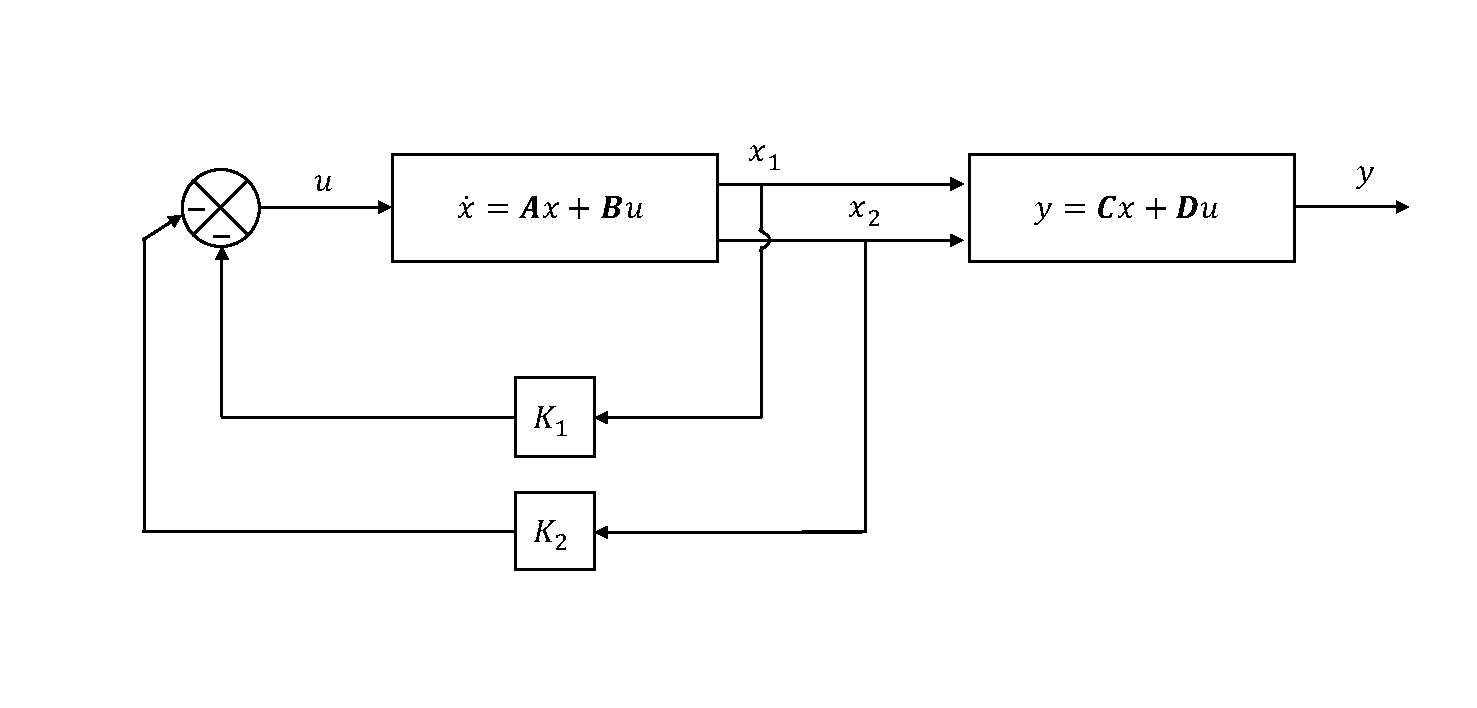
\includegraphics[scale=0.4]{diagrama.pdf}
\caption{LQR controller block diagram}
\label{fig:block_diagram}
\end{figure}

Figure \ref{fig:pendulum_control} shows simulation results with the designed LQR control system when the initial pendulum angle $\theta(0)= 5º \simeq 0.08 rad$. It can be seen how the inverted pendulum system returns to its reference position (zero).

\begin{figure}[!hbt]
\centering
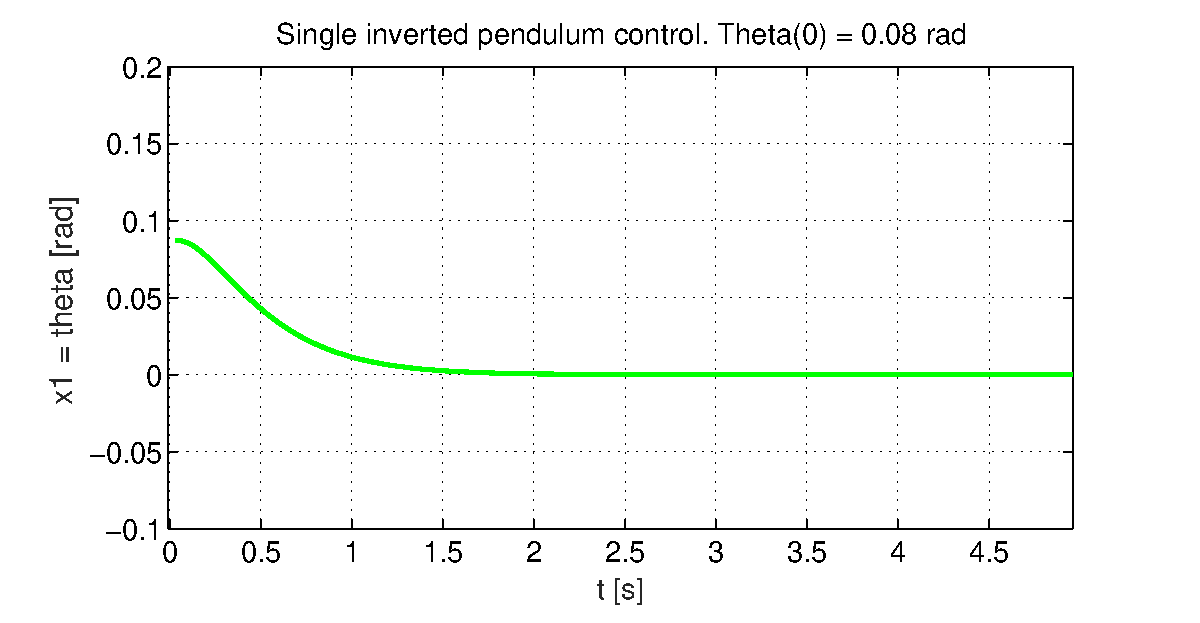
\includegraphics[scale=0.6]{00_single_inverted_pendulum_control.eps}
\caption{Linear inverted pendulum control with initial perturbations.}
\label{fig:pendulum_control}
\end{figure}

The state space representation \ref{eq:state_space}, \ref{eq:state_space_out} is a controllable canonical form that is important for the LQR controller design. It is desired to keep the actual ZMP, measured and computed by force-torque sensors located in the feet of the humanoid robot, close to its stable reference position as was discussed in previous sections. As the system is a type 0 plant, it is necessary to insert an integrator in order to design a ZMP servo control system (type 1) and remove the steady state error. Therefore, we feed the output signal $y$ (which indicates the real ZMP) back to the input and an integrator in the feedforward loop as is shown in Figure \ref{fig:diagrama_int}. Here, $z$ denotes the error between the actual and the reference ZMP, $u$ represents the commanded angle to the system and $u_D$ is the corresponding angle to the reference ZMP ($r$).

\begin{figure}[!hbt]
\centering
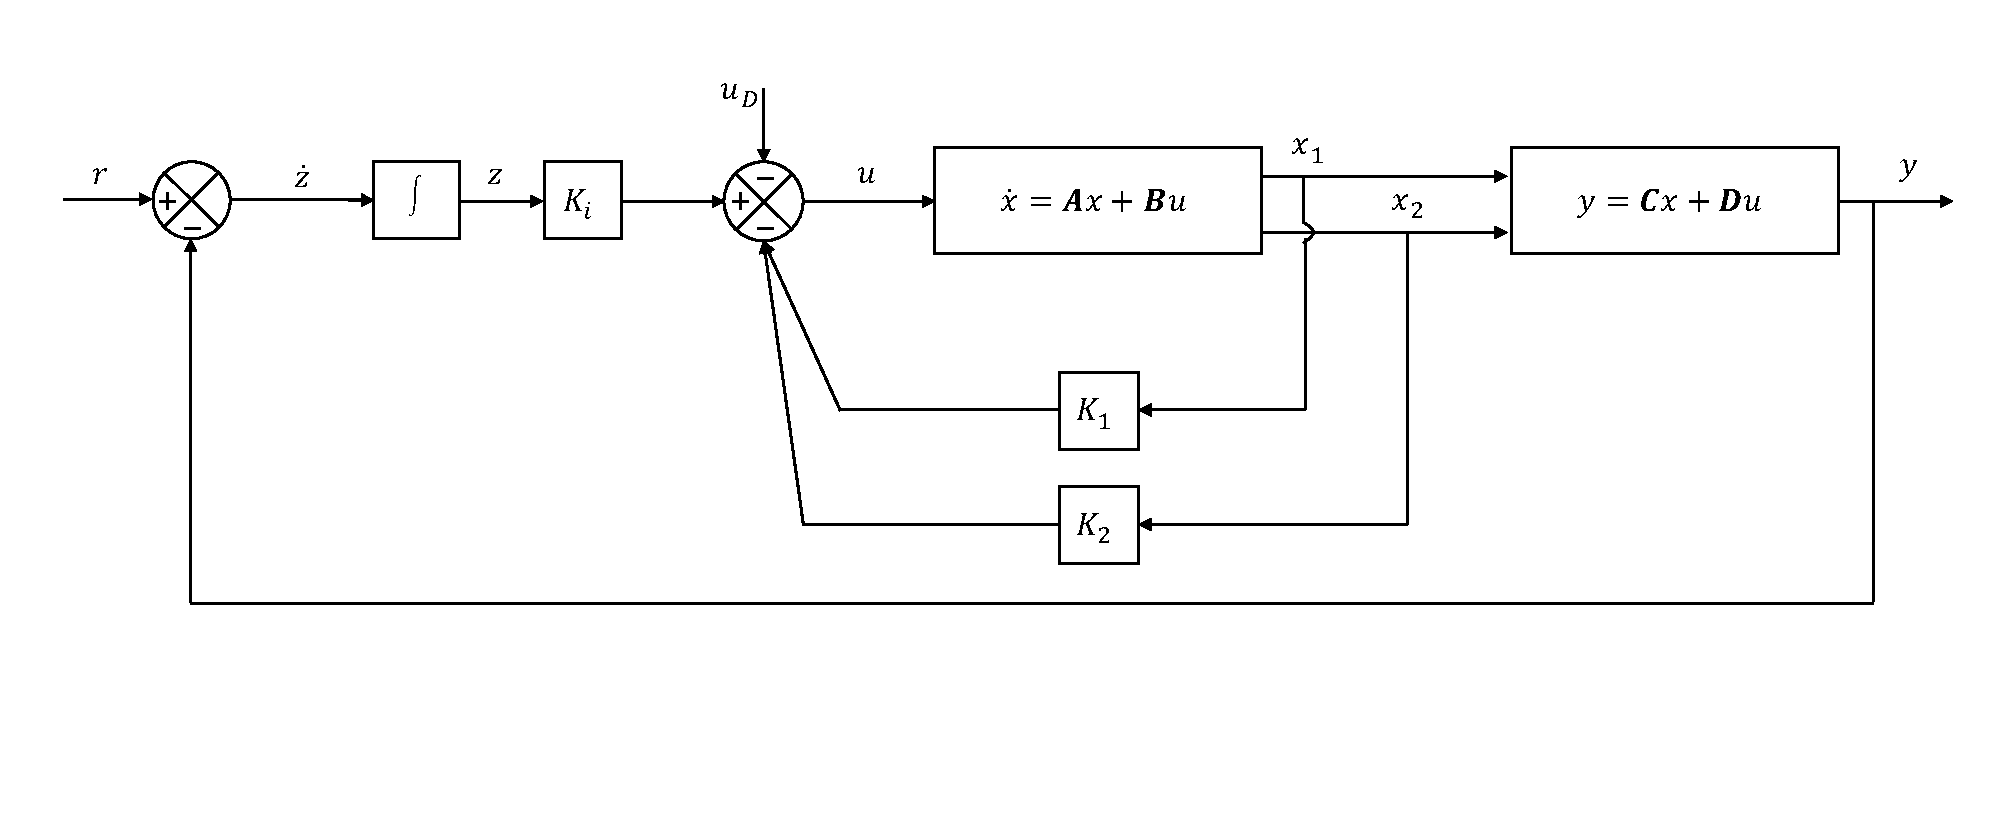
\includegraphics[scale=0.4]{diagrama_int.pdf}
\caption{ZMP LQR control system.}
\label{fig:diagrama_int}
\end{figure}

Thus, referring equations \ref{eq:state_space} and \ref{eq:state_space_out} and Figure \ref{fig:diagrama_int} and considering the actual ZMP position as the output of the system and $r$ as the reference input signal we obtain the equations for the closed loop system as follows:
\begin{equation}
\mathbf{\dot{x}} = \mathbf{A}\textbf{x} + \mathbf{B}u
\end{equation}

\begin{equation}
y = \textbf{C}\textbf{x} + \textbf{D}u
\end{equation}

\begin{equation}
u = - \textbf{K}\textbf{x} + K_i z - K_u u_D
\end{equation}

\begin{equation}
\dot{z} = r - y = r - (\textbf{C}\textbf{x} + \textbf{D}u)
\end{equation}

For the type 1 servo system, the state error equation is given by:
\begin{equation}
\begin{bmatrix}
\dot{\textbf{x}}\\
\dot{z}
\end{bmatrix} = 
\begin{bmatrix}
\textbf{A} & \textbf{0}\\
\textbf{-C} & 0
\end{bmatrix}
\begin{bmatrix}
\textbf{x}\\
z
\end{bmatrix} + 
\begin{bmatrix}
\textbf{B}\\
0
\end{bmatrix}
u
\end{equation}
and the control signal $u$ is given by:
\begin{equation}
u = \begin{bmatrix}
-\textbf{K} & K_i
\end{bmatrix}
\begin{bmatrix}
\textbf{x}\\
z 
\end{bmatrix}
- K_u u_D
\end{equation}

Figure \ref{fig:step_response} shows simulation results with the designed LQR control system with an integrator in the direct control loop. One can see how the output $y$ reaches the step reference of ZMP. Note that the output goes to negative values when the reference suddenly changes its value. This abrupt change makes the output derivative to reach higher values, so it can be solved reducing the abrupt change of the reference signal, i.e., using a ramp signal instead of a step. In Figure \ref{fig:ramp_response} the reference change is smaller and the output is smoother.

\begin{figure}[!hbt]
\centering
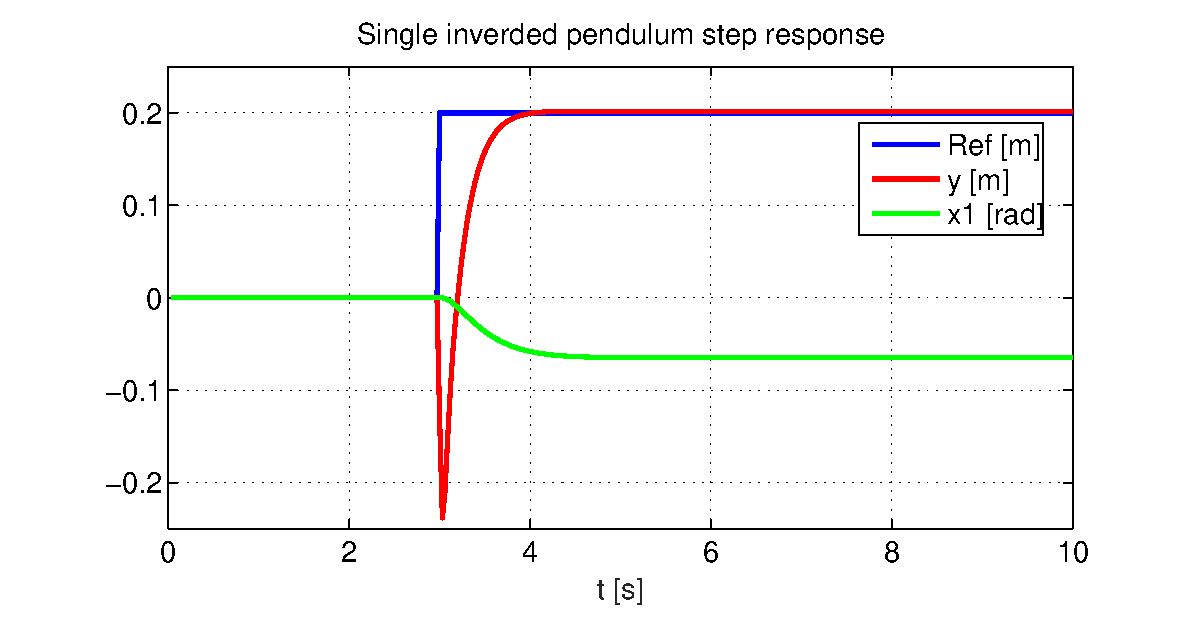
\includegraphics[scale=0.6]{010_step_response.eps}
\caption{Linear inverted pendulum step response.}
\label{fig:step_response}
\end{figure}

\begin{figure}[!hbt]
\centering
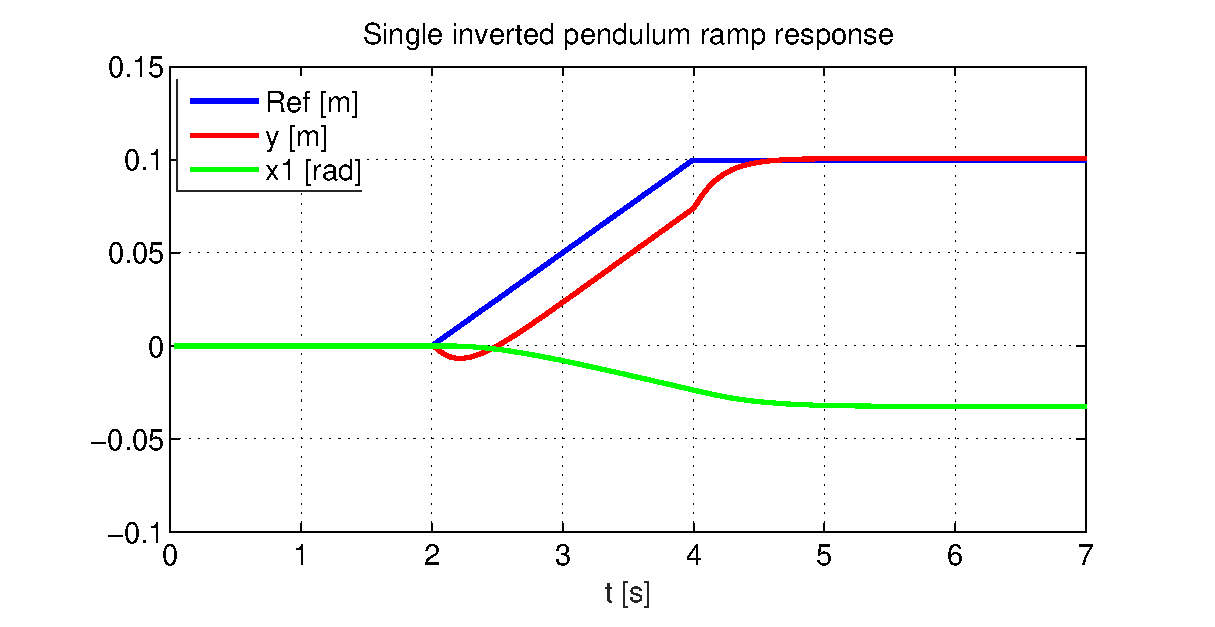
\includegraphics[scale=0.6]{011_ramp_response.eps}
\caption{Linear inverted pendulum \textcolor{red}{smooth} step response.}
\label{fig:ramp_response}
\end{figure}









\section{Stabilizer}
Previously it was shown that the dynamics of a humanoid robot can be a single inverted pendulum and how the pendulum maintains a desired position thanks to the controller designed. Now, let us introduce the detailed stabilizer structure (Figure \ref{fig:stabilizer}).

\begin{figure}[!h]
\centering
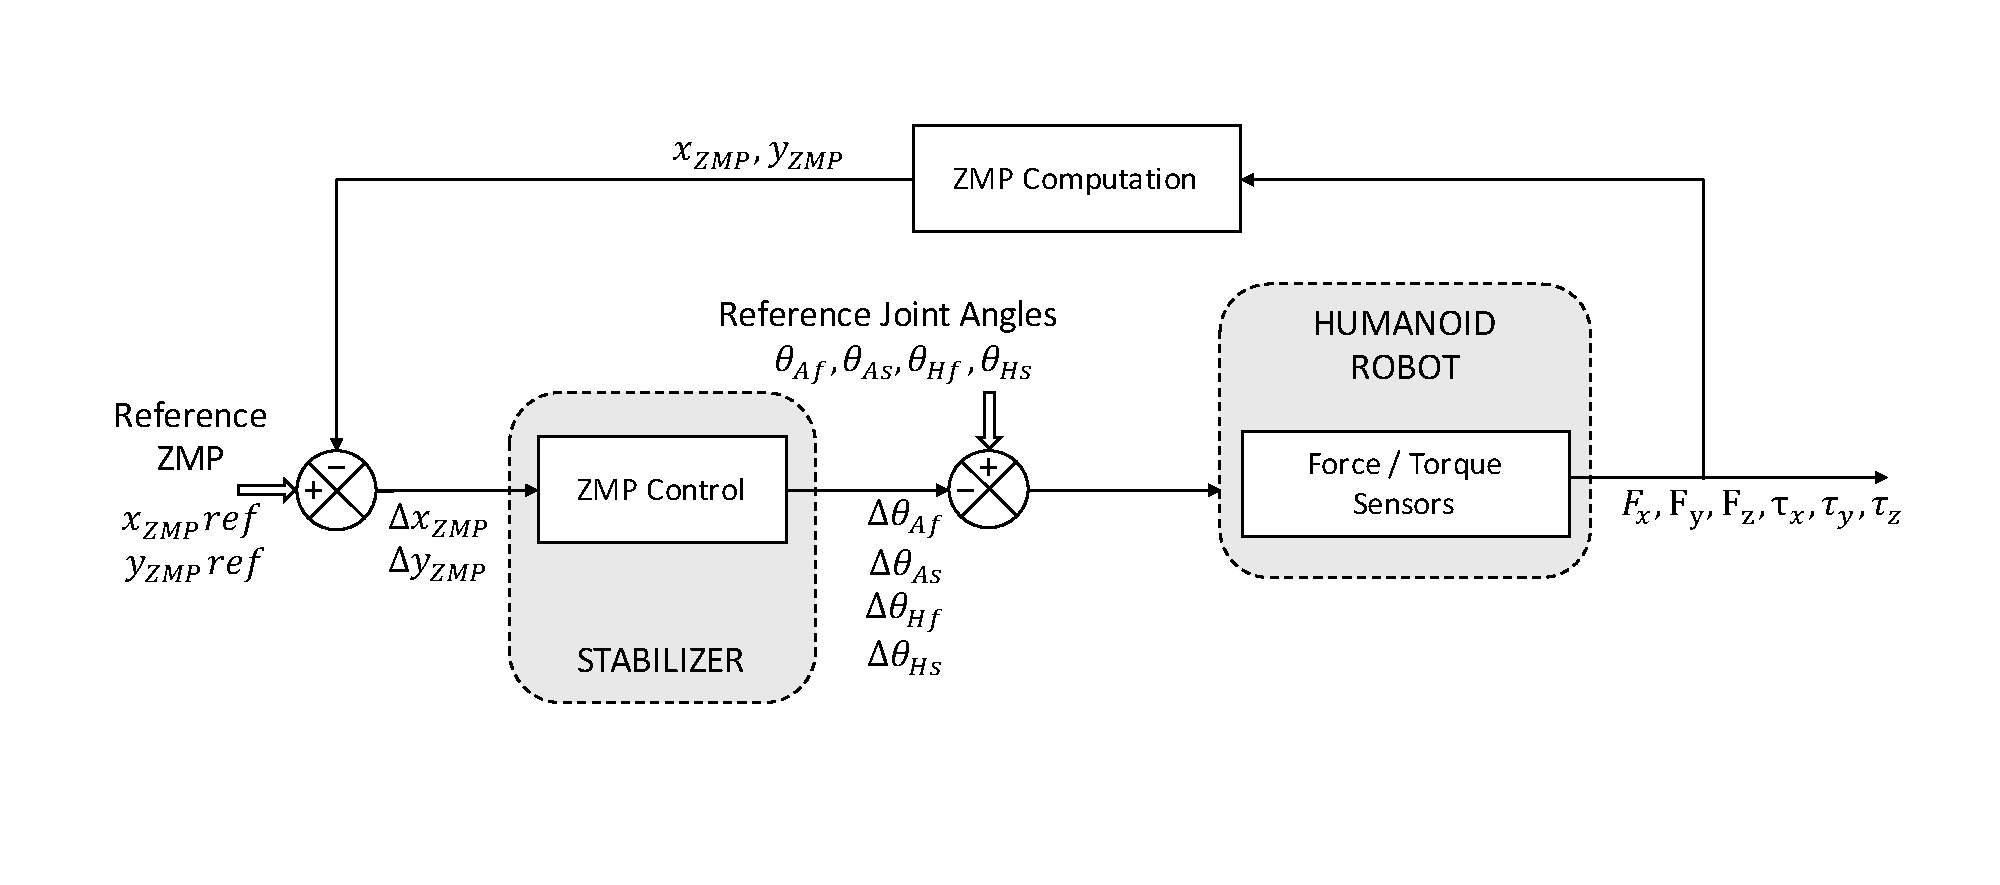
\includegraphics[scale=0.4]{stabilizer.pdf}
\caption{Stabilizer architecture.}
\label{fig:stabilizer}
\end{figure}

The sensorial system of the robot consisting of two six-axis force-torque sensors located at the robot ankles, provide the controller the real distribution of the forces and torques $F_x$, $F_y$, $F_z$, $\tau_x$, $\tau_y$, $\tau_z$ at the contact point of the foot with the ground. After the actual ZMP position $x_{ZMP}$, $y_{ZMP}$ is computed, the ZMP errors ($\Delta x_{ZMP}$, $\Delta y_{ZMP}$) can be estimated. These errors are the input data for the Stabilizer and it controls the error in ZMP positioning of the humanoid robot by the motion of the ankle joints.


\section{Control strategies}
Humans are capable of performing numerous dynamical movements in a wide variety of complex and novel environments while robustly rejecting a large spectrum of disturbances. Human movements such as a forward step and rapid arm rotations allow them to maintain overall balance in non-stability situations. Many researchers have studied how humans unwittingly use their body parts to recover balance as a response of external disturbances and make an approach for studying the stability of humanoid robots.

When the humanoid robot is in a stable posture, perturbantions may appear and they can be classified according the direction of action of that perturbations. All of them can be decomposed in anteroposterior disturbances (sagittal plane) and mediolateral disturbances (frontal plane). Studies of quiet stance have suggested separate postural strategies for balance in both planes depending on the stance position \cite{Winter1996}. There are three main mechanisms that can be applied to regain balance in such planes depending on the level of the disturbance: ankle, hip and step strategies.

The first is the ankle strategy. This strategy is applied in the sagittal plane or anteroposterior disturbances. For low intensity disturbances, the body can be considered as a nearly stiff pendulum, and balance adjustmensts are mainly made in the ankle joint, with the body balancing like a single inverted pendulum (Nashner, 1985). 

In the hip strategy, the resulting motion is mainly applied to the hip joints (Horak, et al. 1990). It can be applied independently or in combination of the ankle strategy. The hip joint movement is triggered when the external disturbance increases and the ankle strategy is not enough to keep balance. The hip strategy, same as ankle one, acts in the anteroposterior direction.

The last one is the step strategy. When these postural corrections become insufficient, the base of support must be adjusted (Carr, et al. 1987; Horak, et al. 1990). The modification of the support base leads new balance stability limits.

Figure (¿?) sumarizes this three strategies and Figure \ref{fig:strategies} shows the levels for strategy triggering. These limits are not fixed and they depend of the humanoid design as the sole surface or the height of the whole body, environmental conditions, i. e, standing in a flat surface has different strategy limits than in a narrow surface.

\begin{figure}[!htbp]
\centering
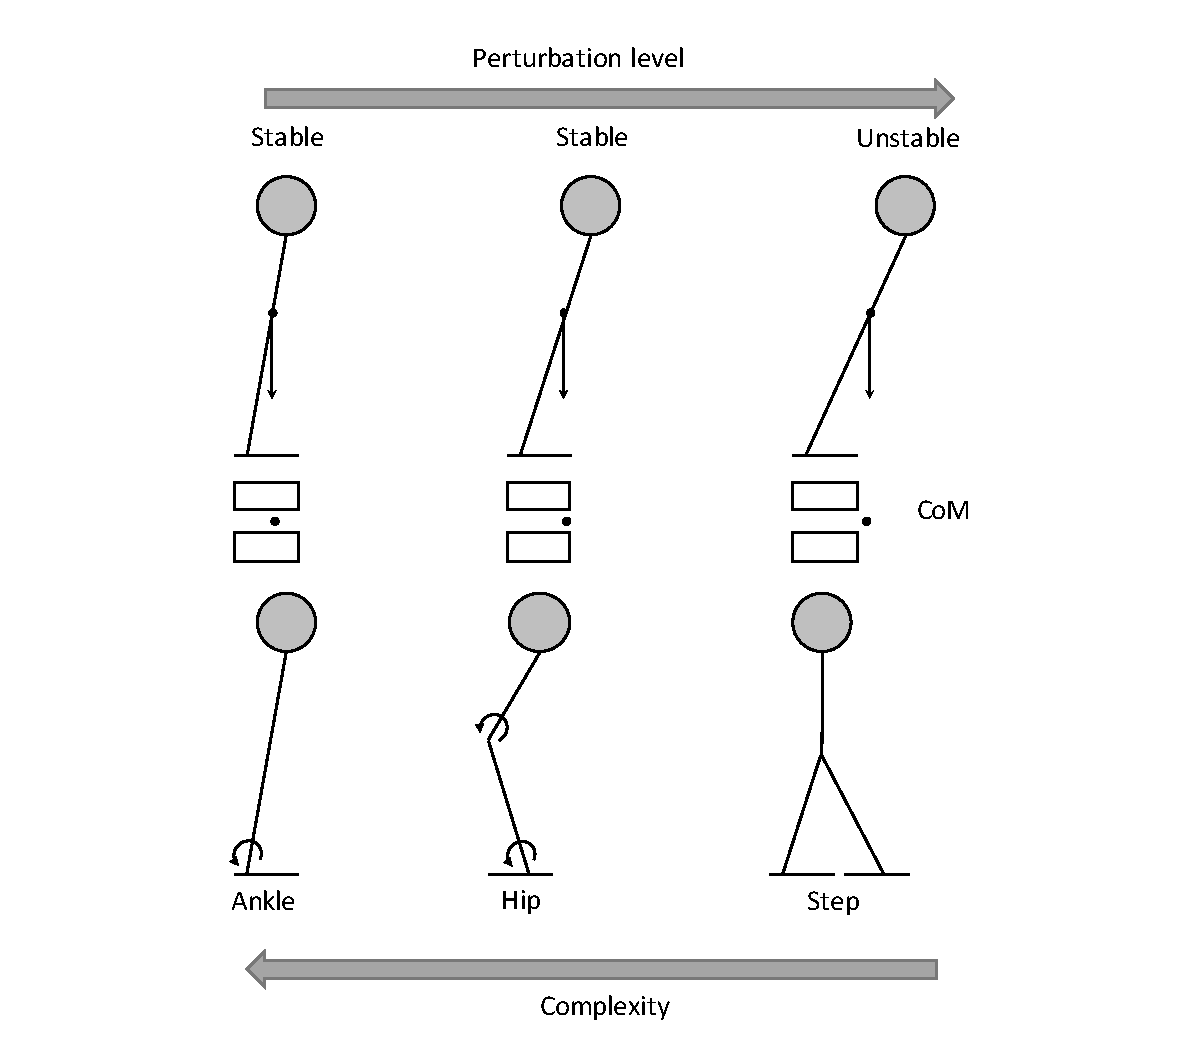
\includegraphics[scale=0.5]{strategies.pdf}
\caption{Recovery strategies.} \label{fig:strategies}
\end{figure}

In the mediolateral direction or frontal plane, the disturbances are compensated by the lateral movement of the hip joint in the case of upright stance. Double support in frontal plane, means there are two support points and a pendulum can not be considered. Both legs and the trunk of the robot make a parallelogram with the ground (see Figure \ref{fig:piernas} (a)). If a disturbance appears, and the hips maintain their perpendicular angles to the body, the feet will begin to loose contact with the ground as shown in Figure \ref{fig:piernas} (b). Then, to maintain stability, the angles of the parallelogram must keep on their relationship without loosing contact between feet and the ground, and the motion is applied to ankle and hip joints (Figure \ref{fig:piernas} (c)). 


\begin{figure}[!htbp]
\centering
\subfigure[]{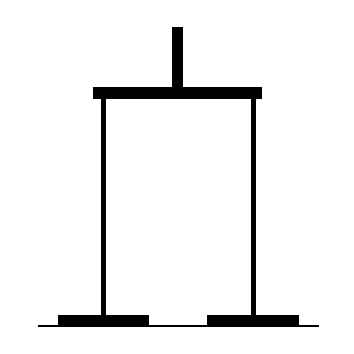
\includegraphics[width=40mm]{piernas1.pdf}}
\subfigure[]{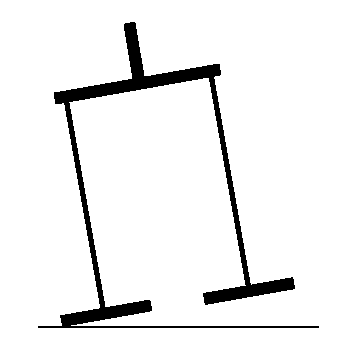
\includegraphics[width=40mm]{piernas2.pdf}}
\subfigure[]{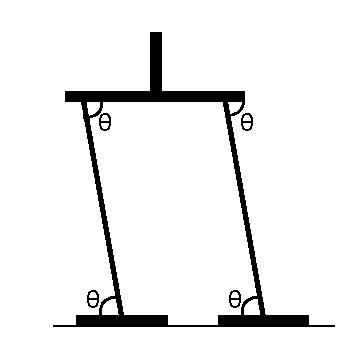
\includegraphics[width=40mm]{piernas3.pdf}}
\caption{Influence of hip and ankle angles in the frontal plane stability.} \label{fig:piernas}
\end{figure}





\chapter{Experimental results}
In this chapter the experimental results are presented and discussed. All the experiments have been executed on TEO humanoid robot.

\section{ZMP computation}
Using F-T sensors located at the ankles of the robot, the ZMP values are obtained from equations \eqref{eq:xzmp} and \eqref{eq:yzmp}, where the distance between the ground and the sensor center is 194 milimeters (sensor height is obtained from \textcolor{red}{APPENDIX: planes}).

Data read form de Data Acquisition Card is scaled to SI units, clustered to a YARP Bottle object and sent through YARP ports. Each sensor rate is about $20 \mu s$, thus four sensors reading rate is about $80 \mu s$. The problem comes when the data is sent trough YARP ports and there is a client receiving and processing this data. Then the update rate hugely decreases to $10 - 50 ms$, deppending on the reader processing cycle. That occurs because 
%the default YARP behaviour is to send data when the client is free. That means that data is received befor any processing is donw by the client. If updates arrive faster than processing occurs, then updates will be lost from time to time, but the most recen update received will always be available to the client inmediately when processing is completed.

the arrival of updates is delayed until the client completes processing and no updates will ever be lost on the client side \cite{Yarp2006}.


For a visual point of view, it has been developed a Python application using the module \textit{Matplotlib} to represent the ZMP in a plane representation of the ground and the sole borders in both single and double support. The ZMP stability areas are also represented according to the limits obtained later in section \textcolor{red}{section} as shown in Figure \textcolor{red}{FIGURA: dos imagenes de single y double support con las areas pintadas.}

\nocite{*}
\bibliographystyle{apacite}
\bibliography{library}

\end{document}

